\documentclass[a4paper,12pt]{article}
\usepackage{test,caption,subcaption,tikz}
\usetikzlibrary{decorations.pathreplacing,calligraphy}
\usepackage[colorlinks,citecolor=blue,urlcolor=magenta]{hyperref}

\usepackage[backend = bibtex8,
style=authoryear-comp, % for author-year compact format
sorting=nyt, % sort by name, year, title
dashed=false, % don't use dash for repeated author
maxcitenames=2, % maximum names to cite in text
maxbibnames=99, % maximum names to list in reference
uniquelist=false,
uniquename=init,
giveninits=true, % first name initials
natbib, % use natbib commands
date=year % year only
]{biblatex}
\addbibresource{localbib.bib}

\DeclareFieldFormat{pages}{#1} % suppress pp.
\renewbibmacro{in:}{\ifentrytype{article}{}{\printtext{\bibstring{in}\intitlepunct}}} % delete In:

\newcommand{\AAT}[1]{{\color{magenta} AAT: #1}}
\renewcommand{\TH}[1]{{\color{magenta} TH: #1}}

\usepackage[inline,shortlabels]{enumitem}
\setlist[enumerate,1]{label=(\roman*)}

\usepackage[margin = 1.25in]{geometry}
\usepackage{setspace}
\onehalfspacing

%opening
\title{A Theory of Rational Housing Bubbles with Phase Transitions}
\author{Tomohiro Hirano\thanks{Department of Economics, Royal Holloway, University of London. Email: \href{mailto:tomohiro.hirano@rhul.ac.uk}{tomohih@gmail.com}.} \and Alexis Akira Toda\thanks{Department of Economics, University of California San Diego. Email: \href{mailto:atoda@ucsd.edu}{atoda@ucsd.edu}.}}

\numberwithin{equation}{section}
\numberwithin{thm}{section}

% define custom commands
\newcommand{\cE}{\mathcal{E}}
\newcommand{\cS}{\mathcal{S}}

\begin{document}

\maketitle

\begin{abstract}

Empirically observed rent-price ratios suggest a disconnection between fundamentals and prices. We analyze equilibrium housing prices in an overlapping generations model with perfect housing and rental markets. We prove that the economy exhibits a two-stage phase transition: as the income of home buyers rises, the equilibrium regime changes from fundamental only to coexistence of fundamental and bubbly equilibria. With even higher incomes, fundamental equilibria disappear and housing bubbles become inevitable. Expectation-driven housing booms containing a bubble and their collapse can occur. Contrary to widely-held beliefs, fundamental equilibria in the coexistence region are inefficient despite housing being a productive non-reproducible asset.

\medskip

\textbf{Keywords:} bubble, expectations, housing, phase transition, welfare.

\medskip

\textbf{JEL codes:} D53, G12, R21.
\end{abstract}

\section{Introduction}

Imagine a simple world in which housing rents (which can be thought of as dividends of housing) grow at a constant rate $g$ and agents discount future cash flows at rate $\delta>g$. Then a simple present value calculation yields the linear relationship $P=r/(\delta-g)$ between rent $r$ and housing price $P$,\footnote{$P=\int_0^\infty \e^{-\delta t}r\e^{gt}\diff t=r/(\delta-g)$.} so log rent and log price should have a linear relationship with a coefficient of 1 regardless of the rent growth rate $g$ or the discount rate $\delta$. Figure \ref{fig:rent_price} shows this relation across U.S. counties for 2019. Although there is a positive association, the coefficient is significantly above 1, implying that in high-rent areas like San Diego, housing prices tend to be disproportionately more expensive. But this could be an artefact of omitted variables: for instance if high-rent areas also have high rent growth, the price could be disproportionately high. To examine this point, we can rewrite the present value formula as $g=\delta-r/P$. Therefore under rational expectations, the initial rent-price ratio $r/P$ (the ``rent yield'') and the subsequent rent growth $g$ should have a linear relationship with a coefficient of $-1$. Figure \ref{fig:yield_rentg} shows this relation across U.S. counties, where the initial year is 2016 and the rent growth is averaged over the 2016--2022 period. Although there is a negative association, the coefficient is significantly smaller than 1 in absolute value.

\begin{figure}[htb!]
\centering
\begin{subfigure}{0.48\linewidth}
    \includegraphics[width=\linewidth]{figures/fig_rent_price.pdf}
    \caption{Rent and housing price.}\label{fig:rent_price}
\end{subfigure}
\begin{subfigure}{0.48\linewidth}
    \includegraphics[width=\linewidth]{figures/fig_yield_rentg.pdf}
    \caption{Rent-price ratio and rent growth.}\label{fig:yield_rentg}
\end{subfigure}
\caption{Housing rent and price across U.S. counties, 2016--2022.}\label{fig:county}
\caption*{\footnotesize See Appendix \ref{sec:data} for detailed explanation.}
\end{figure}

The present value model as well as the empirical analysis presented above are obviously far too simplistic as it ignores many factors.\footnote{For instance, if housing is subject to a property tax at rate $\tau$, then the discount rate $\delta$ needs to be modified to $\delta+\tau$. However, if we include state dummy variables in the regression of Figure \ref{fig:yield_rentg} to absorb state-specific effects such as property taxes and local economic conditions, the coefficient further decreases in magnitude to $-0.13$.} However, these figures do suggest that it may not be so simple to explain the connection between fundamentals (rents) and housing prices using a standard asset pricing model. Motivated by this observation, in this paper we theoretically study the (dis)connection between fundamentals and housing price---the possibility and inevitability of housing bubbles---in a rational general equilibrium model.

To theoretically analyze rational housing bubbles in the simplest setting, we consider a stylized overlapping generations (OLG) model with a consumption good, housing stock, and housing service traded at perfect housing and rental markets. The agents live for two periods (young and old age), consume the good in both periods, and live in a house when transitioning from young to old. The ownership and occupancy of a house are separated, so there is a price for house ownership as a financial asset (housing price) and a price for house occupancy as a commodity (rent). A competitive equilibrium consists of a sequence of prices (housing price and rent) and allocations (consumption good, housing stock, and housing service) such that all agents optimize and markets clear. In this model, the dividend of housing, namely rent, is endogenously determined by the demand and supply of housing. If housing supply is constant, as the economy grows and agents get richer, they increase the demand for housing, which pushes up both the housing price and rent. Under these circumstances, it is not obvious whether house prices will grow faster than rents and a housing bubble emerges. Therefore the possibility or inevitability of housing bubbles becomes a nontrivial theoretical question.

In this setting, we obtain three main results.  First, we theoretically identify conditions under which the equilibrium housing price reflects the fundamentals in the long run or exhibits a bubble. We prove that the economy experiences a two-stage phase transition. When the long run income ratio of the young (home buyers) is sufficiently low, housing bubbles cannot arise and a fundamental equilibrium exists. When the ratio rises and exceeds the first critical value, a phase transition occurs. Both a fundamental and a bubbly equilibrium exist, and the equilibrium is selected by agents' self-fulfilling expectations. When the income ratio exceeds the second and still higher critical value, another phase transition takes place. The fundamental equilibrium ceases to exist and only a bubbly equilibrium exists. In other words, bubbles are inevitable for the existence of equilibrium. Furthermore, we prove the uniqueness of equilibrium under weak conditions. We show that the fundamental equilibrium is always unique, and the bubbly equilibrium is unique if the elasticity of intertemporal substitution is not too much below $1/2$.

The intuition for this two-stage phase transition is the following. Let $G>1$ be the long run growth rate of the economy and $\gamma>0$ be the reciprocal of the elasticity of substitution between consumption and housing. Empirical estimates suggest $\gamma\le 1$,\footnote{\label{fn:elasticity}\citet[Table 2]{OgakiReinhart1998} estimate the elasticity of substitution between durable and nondurable goods using aggregate data and obtain a point estimate of 1.24. \citet[Appendix C]{PiazzesiSchneiderTuzel2007} estimate a cointegrating equation between the relative price and quantity of housing consumption using aggregate data and obtain an elasticity of 1.27. \citet{DavisOrtalo-Magne2011} document that the expenditure shares on housing are constant over time and across U.S. metropolitan statistical areas (MSA), which suggests an elasticity of 1.} and a theoretical argument also supports it: if $\gamma>1$, as the economy grows and agents get richer, the young asymptotically spend all income on housing, the price-rent ratio converges to zero, and the interest rate diverges to infinity, which are all pathological. Since $\gamma=1$ (Cobb-Douglas) is a knife-edge case, it is natural to focus on the case $\gamma<1$. Under this condition, by equating marginal utility to prices, consumption grows at rate $G$ but the rent grows at rate $G^\gamma<G$. Therefore, if the housing price only reflects the fundamentals in the long run equilibrium, it must also grow at rate $G^\gamma$. Since housing price grows slower than endowments in any fundamental equilibrium, the economy becomes ``house-less'' in the long run and the interest rate $R$ is pinned down as the marginal rate of intertemporal substitution in the autarky allocation. If $R>G^\gamma$, a fundamental equilibrium exists. If $R<G^\gamma$, a fundamental equilibrium cannot exist, for otherwise the fundamental value of housing becomes infinite, which is obviously impossible in equilibrium. Therefore as the young become richer and the interest rate falls below a certain threshold, a fundamental equilibrium becomes unsustainable, and a housing bubble inevitably emerges. In the long run equilibrium with housing bubbles we must have $R=G$ so that the bubble is just sustainable. Fundamental and bubbly equilibria coexist when the autarkic interest rate satisfies $G^\gamma<R<G$, which corresponds to an intermediate range for the income ratio of the young.

As our second main result, using the two-stage phase transition and uniqueness of equilibrium dynamics, we present expectation-driven housing booms containing a bubble and their collapse. In our model, because agents are forward-looking and housing prices reflect information about future economic conditions, whether bubbles arise or not in equilibrium depends on long run expectations about the income ratio of home buyers. As long as agents expect high incomes in the future, housing prices start rising now and contain a bubble, even if the current income of home buyers is low and the economy appears to stay in the fundamental region. During this dynamics driven by optimistic beliefs, the price-income ratio and the price-rent ratio simultaneously rise, and hence the housing price dynamics may appear unsustainable because prices grow faster than incomes. On the other hand, if these optimistic expectations do not materialize, the bubble collapses.

Our third main result is the welfare analysis. It has been widely believed in the literature that the introduction of a productive non-reproducible asset like land eliminates the dynamic inefficiency in overlapping generations models. We theoretically show that this is not necessarily true: inefficient equilibria can still occur even though the housing and rental markets in our model are perfectly competitive and frictionless. In the region where fundamental and bubbly equilibria coexist, we prove that the bubbly equilibrium is efficient but the fundamental equilibrium is not. Therefore policymakers may have a role in guiding expectations and equilibrium selection.

The rest of the paper is organized as follows. Section \ref{sec:prelim} presents the model, derives equilibrium conditions, and defines a housing bubble. Section \ref{sec:eq} establishes the existence of equilibria and study the long run behavior of equilibrium housing prices. Sections \ref{sec:phase} and \ref{sec:welfare} discuss the two-stage phase transition and welfare implications of housing bubbles. Section \ref{sec:discuss} discusses testable implications and the related literature. The proofs of the main results are deferred to Appendix \ref{sec:proof}.

\section{Preliminaries}\label{sec:prelim}

\subsection{Model}\label{subsec:prelim_model}

Time is discrete and indexed by $t=0,1,\dotsc$. We consider a deterministic overlapping generations (OLG) economy in which agents live for two periods (young and old age) and demand a consumption good and housing service. We employ an OLG model because it allows us to capture life-cycle behaviors regarding housing demand in a simple setting.

\paragraph{Commodities, asset, and endowments}

There are two perishable commodities (consumption good and housing service) and a durable non-reproducible asset (housing stock) in the economy. The housing service is the right to occupy a house between two periods. Every period, one unit of housing stock inelastically produces one unit of housing service.\footnote{It is important to distinguish the housing service from the housing stock. An analogy is that the consumption good is an apple, housing service is a banana, and housing stock is a banana tree.} The time $t$ endowment of the consumption good is $a_t>0$ for the young and $b_t>0$ for the old. At $t=0$, the housing stock (whose aggregate supply is normalized to 1) is owned by the old.

\paragraph{Preferences}

An agent born at time $t$ lives for two periods and has utility function $U(y_t,z_{t+1},h_t)$, where $y_t>0$ is consumption when young, $z_{t+1}>0$ is consumption when old, and $h_t>0$ is housing service consumed when transitioning from young to old. As usual, we assume that $U:\R_{++}^3\to \R$ is continuously differentiable, has strictly positive first partial derivatives, is strictly quasi-concave, and satisfies Inada conditions to guarantee interior solutions. The initial old care only about their consumption $z_0$.

\paragraph{Markets}

We consider an ideal world in which the ownership and occupancy of housing are separated and traded at competitive frictionless markets: agents trade housing (a financial asset) only to store value (transfer resources across time), whereas they purchase housing service (a commodity) only to derive utility.\footnote{Therefore nothing prevents agents from purchasing a mansion as an investment while renting a campsite to sleep, or vice versa. Owner-occupants can be thought of agents who rent the houses they own to themselves. The literature sometimes stresses the indivisibility of housing stock and nontradability of dividends \citep[p.~1568]{PiazzesiSchneider2016}. While these imperfections could be important, they are likely less so compared to the past due to the development of real estate investment trusts (REITs) and vacation rentals like Airbnb. However, because in our model agents within a generation are homogeneous, in equilibrium each young agent demands one unit of housing and one unit of housing service, so the agents end up being owner-occupants.}

Let $r_t$ be the price of housing service (rent) and $P_t$ be the housing price (excluding current rent) quoted in units of time $t$ consumption. Let $x_t$ denote the demand for the housing stock. Then the budget constraints of an agent born at time $t$ are
\begin{subequations}\label{eq:budget}
\begin{align}
    &\text{Young:} & y_t+P_tx_t+r_th_t&\le a_t, \label{eq:budget_young}\\
    &\text{Old:} & z_{t+1}&\le b_{t+1}+(P_{t+1}+r_{t+1})x_t.\label{eq:budget_old}
\end{align}
\end{subequations}
The budget constraint of the young \eqref{eq:budget_young} states that the young spend income on consumption, purchase of housing stock, and rent. The budget constraint of the old \eqref{eq:budget_old} states that the old consume the endowment and the income from renting and selling housing.

\paragraph{Equilibrium}

As usual, an equilibrium is defined by individual optimization and market clearing.

\begin{defn}\label{defn:eq}
A competitive equilibrium consists of a sequence of prices $\set{(P_t,r_t)}_{t=0}^\infty$ and allocations $\set{(y_t,z_t,h_t,x_t)}_{t=0}^\infty$ such that for each $t$,
\begin{enumerate}
    \item (Individual optimization) The young maximize utility $U(y_t,z_{t+1},h_t)$ subject to the budget constraints \eqref{eq:budget},
    \item (Commodity market clearing) $y_t+z_t=a_t+b_t$,
    \item (Rental market clearing) $h_t=1$,
    \item (Housing market clearing) $x_t=1$.
\end{enumerate}
\end{defn}

\subsection{Equilibrium conditions}\label{subsec:prelim_eqcond}

We derive equilibrium conditions. Using the rental and housing market clearing conditions $h_t=x_t=1$ and the budget constraint \eqref{eq:budget}, we obtain
\begin{equation}
    (y_t,z_t)=(a_t-P_t-r_t,b_t+P_t+r_t)=(a_t-S_t,b_t+S_t), \label{eq:yz}
\end{equation}
where $S_t\coloneqq P_t+r_t$ is total expenditure on housing. Throughout the paper, we refer to $P_t$ as the housing price and $S_t$ as the housing expenditure. Let
\begin{equation}
R_t\coloneqq \frac{P_{t+1}+r_{t+1}}{P_t} \label{eq:R}
\end{equation}
be the implied gross risk-free rate between time $t$ and $t+1$. Then the two budget constraints in \eqref{eq:budget} can be combined into one as
\begin{equation}
    y_t+\frac{z_{t+1}}{R_t}+r_th_t\le a_t+\frac{b_{t+1}}{R_t}.\label{eq:budget_combined}
\end{equation}
Letting $\lambda_t\ge 0$ be the Lagrange multiplier associated with the combined budget constraint \eqref{eq:budget_combined}, we obtain the first-order conditions
\begin{subequations}\label{eq:foc}
    \begin{align}
        U_y&=\lambda_t, \label{eq:foc_y}\\
        U_z&=\lambda_t/R_t, \label{eq:foc_z}\\
        U_h&=\lambda_tr_t, \label{eq:foc_h}
    \end{align}
\end{subequations}
where $U_y=\partial U/\partial y$ etc.\ and the utility function is evaluated at
\begin{equation}
(y_t,z_{t+1},h_t)=(a_t-S_t,b_{t+1}+S_{t+1},1).\label{eq:demand}
\end{equation}
Combining \eqref{eq:foc_y} and \eqref{eq:foc_z}, we obtain
$1/R_t=U_z/U_y$. Combining \eqref{eq:foc_y} and \eqref{eq:foc_h}, we obtain $r_t=U_h/U_y$. Combining these two equations, the definition of $R_t$ in \eqref{eq:R}, and $S_t=P_t+r_t$, we may derive an equation that involves only $S_t$ and $S_{t+1}$. Therefore we obtain the following characterization of equilibrium as a solution to a one-dimensional nonlinear difference equation.

\begin{prop}[Equilibrium characterization]\label{prop:eq}
A competitive equilibrium exists if and only if there exists a sequence $\set{S_t}_{t=0}^\infty$ satisfying $0<S_t<a_t$ and
\begin{equation}
    S_{t+1}U_z=S_tU_y-U_h,\label{eq:s_dynamics}
\end{equation}
where the partial derivatives of $U$ are evaluated at \eqref{eq:demand}. Under this condition, the equilibrium consumption, housing price, rent, and risk-free rate are given by
\begin{subequations}\label{eq:eqobj}
\begin{align}
    (y_t,z_t)&=(a_t-S_t,b_t+S_t), \label{eq:eq_yz}\\
    P_t&=S_t-(U_h/U_y)(a_t-S_t,b_{t+1}+S_{t+1},1), \label{eq:eq_p}\\
     r_t&=(U_h/U_y)(a_t-S_t,b_{t+1}+S_{t+1},1), \label{eq:eq_r}\\
     R_t&=(U_y/U_z)(a_t-S_t,b_{t+1}+S_{t+1},1). \label{eq:eq_R}
\end{align}
\end{subequations}
\end{prop}

By Proposition \ref{prop:eq}, an equilibrium is fully characterized by the sequence of housing expenditure $\set{S_t}_{t=0}^\infty$. For this reason, we often refer to $\set{S_t}_{t=0}^\infty$ as an equilibrium without specifying each object in Definition \ref{defn:eq}.

\subsection{Definition of housing bubble}\label{subsec:prelim_bubble}

Following the standard definition of bubbles in the literature, we define a housing bubble by a situation in which the housing price exceeds its fundamental value defined by the present value of rents. Suppose an equilibrium exists and let $R_t>0$ be the gross risk-free rate. Let $q_t>0$ be the Arrow-Debreu price of date-$t$ consumption in units of date-0 consumption, so $q_0=1$ and $q_t=1/\prod_{s=0}^{t-1}R_s$. Since by definition $q_{t+1}=q_t/R_t$ holds, using \eqref{eq:R} we obtain the no-arbitrage condition
\begin{equation}
    q_tP_t=q_{t+1}(P_{t+1}+r_{t+1}). \label{eq:no-arbitrage}
\end{equation}
Iterating \eqref{eq:no-arbitrage} forward, for all $T>t$ we obtain
\begin{equation}
    q_tP_t=\sum_{s=t+1}^Tq_sr_s+q_TP_T. \label{eq:P_iter}
\end{equation}
Since $q_sr_s\ge 0$, we have $\sum_{s=t+1}^\infty q_sr_s\le q_tP_t$, so we may define the \emph{fundamental value} of housing by the present value of rents
\begin{equation}
    V_t\coloneqq \frac{1}{q_t}\sum_{s=t+1}^\infty q_sr_s. \label{eq:Vt}
\end{equation}
Letting $T\to\infty$ in \eqref{eq:P_iter}, we obtain the limit
\begin{equation}
    0\le \lim_{T\to\infty} q_TP_T=q_t(P_t-V_t). \label{eq:TVC}
\end{equation}
When the limit in \eqref{eq:TVC} equals 0, we say that the \emph{transversality condition} (for asset pricing) holds and the asset price $P_t$ equals its fundamental value $V_t$. When $\lim_{T\to\infty} q_TP_T>0$, we say that the transversality condition fails and the asset price contains a \emph{bubble}. Note that under rational expectations, we have either $P_t=V_t$ for all $t$ or $P_t>V_t$ for all $t$. Throughout the rest of the paper, we refer to an equilibrium with (without) a housing bubble a \emph{bubbly (fundamental) equilibrium}.

\section{Existence of long run equilibria}\label{sec:eq}

In this section we study the long run  behavior of equilibrium housing prices.

\subsection{Assumptions}\label{subsec:eq_asmp}

To make qualitative predictions, we put more structure by specializing the utility function and endowments. For the remainder of the paper, the following restrictions are in force.

\begin{asmp}[Endowments]\label{asmp:G}
There exist $G>1$, $a,b>0$, and $T>0$ such that the endowments are $(a_t,b_t)=(aG^t,bG^t)$ for $t\ge T$.
\end{asmp}

Assumption \ref{asmp:G} implies that in the long run, the economy exogenously grows at rate $G>1$ and the income ratio between the young and old is constant.

\begin{asmp}[Utility]\label{asmp:U}
The utility function takes the form
\begin{equation}
    U(y,z,h)=u(c(y,z))+\phi(h), \label{eq:utility}
\end{equation}
where
\begin{enumerate*}
    \item\label{item:U_c} the composite consumption $c(y,z)$ is homogeneous of degree 1 and quasi-concave,
    \item\label{item:U_u} the utility of composite consumption is $u(c)=\frac{c^{1-\gamma}}{1-\gamma}$ for some $\gamma>0$ ($u(c)=\log c$ if $\gamma=1$), and
    \item\label{item:U_phi} the utility of housing service satisfies $\phi'>0$.
\end{enumerate*}
\end{asmp}

Assumption \ref{asmp:U}\ref{item:U_c} implies that agents (apart from the initial old) care about consumption $(y,z)$ only through the homothetic composite consumption $c(y,z)$, which (together with Assumption \ref{asmp:G}) allows us to study asymptotically balanced growth paths. Assumption \ref{asmp:U}\ref{item:U_u} implies that agents have constant elasticity of substitution $1/\gamma>0$ between consumption and housing service. To see this, consider an agent that maximizes utility $u(c)+\phi(h)$ subject to the budget constraint $c+\rho h\le w$, where $\rho>0$ is the rent measured in units of composite consumption. Letting $\lambda$ be the Lagrange multiplier, the first-order conditions are $c^{-\gamma}=\lambda$ and $\phi'(h)=\lambda \rho$. But in equilibrium we have $h=1$, so $\rho=\phi'(1)c^\gamma$. Log-differentiating both sides, we obtain
\begin{equation*}
    -\frac{\partial \log(h/c)}{\partial \log \rho}=\frac{\partial \log c}{\partial \log \rho}=\frac{1}{\gamma},
\end{equation*}
so the elasticity of substitution between consumption and housing is $1/\gamma$.

Throughout the main text, we focus on the case $\gamma<1$ (so the elasticity of substitution between consumption and housing $1/\gamma$ exceeds 1) and defer the analysis of the case $\gamma\ge 1$ to Appendix \ref{sec:gamma>=1}. There are two reasons for doing so. First, elasticity of substitution above 1 is the empirically relevant case (Footnote \ref{fn:elasticity}). Second, as we show in Proposition \ref{prop:gamma>1}, the equilibrium with $\gamma>1$ is pathological: the young asymptotically spend all income on housing (purchase and rent); the price-rent ratio converges to zero; and the gross risk-free rate diverges to infinity, which are all counterfactual. Hence the case $\gamma>1$ is economically irrelevant.

Since by Assumption \ref{asmp:U}\ref{item:U_c} $c$ is homogeneous of degree 1 and quasi-concave, Theorem 3 of \citet[p.~208]{Berge1963} implies that $c$ is actually concave. Because we wish to study smooth interior solutions, we further strengthen the assumption as follows.

\begin{asmp}[Composite consumption]\label{asmp:c}
The composite consumption $c:\R_{++}^2\to (0,\infty)$ is homogeneous of degree 1, twice continuously differentiable, and satisfies $c_y>0$, $c_z>0$, $c_{yy}<0$, $c_{zz}<0$, $c_y(0,z)=\infty$, $c_z(y,0)=\infty$.
\end{asmp}

A typical functional form for $c$ satisfying Assumption \ref{asmp:c} is the constant elasticity of substitution (CES) specification
\begin{equation}
    c(y,z)=\begin{cases*}
        ((1-\beta)y^{1-\sigma}+\beta z^{1-\sigma})^\frac{1}{1-\sigma} & if $0<\sigma\neq 1$,\\
        y^{1-\beta}z^\beta & if $\sigma=1$,
        \end{cases*} \label{eq:CES}
\end{equation}
where $1/\sigma$ is the elasticity of intertemporal substitution and $\beta\in (0,1)$ dictates the time preference.

In the subsequent analysis, we first focus on the long run behavior of the economy and then examine transitional dynamics driven by expectations. We present two simple lemmas that are useful for this purpose.

\begin{lem}[Backward induction]\label{lem:backward}
    Suppose Assumptions \ref{asmp:U} and \ref{asmp:c} hold. If there exists an equilibrium $\cS_T=\set{S_t}_{t=T}^\infty$ starting at $t=T$, there exists a unique equilibrium $\cS_0=\set{S_t}_{t=0}^\infty$ starting at $t=0$ that agrees with $\cS_T$ for $t\ge T$.
\end{lem}

Lemma \ref{lem:backward} shows that once we establish the existence of an equilibrium for an economy starting at large enough $t$ (\eg, close to the steady state), the existence of an equilibrium starting at $t=0$ is immediate. This lemma allows us to focus on the long run behavior of the economy and guarantees the uniqueness of the transitional dynamics. Since by Assumption \ref{asmp:G} the endowments eventually grow at a constant rate $G$, unless otherwise specified, without loss of generality we assume that endowments are given by $(a_t,b_t)=(aG^t,bG^t)$ for all $t$.

The following lemma bounds the equilibrium rents.

\begin{lem}[Bounds on rents]\label{lem:r_bound}
Suppose Assumptions \ref{asmp:G}--\ref{asmp:c} hold, $\gamma<1$, and let $\set{S_t}_{t=0}^\infty$ be an equilibrium. Then the following statements are true.
\begin{enumerate}
    \item There exists $\bar{r}>0$ such that $r_t\le \bar{r}G^{\gamma t}$ for all $t$.
    \item If $\limsup_{t\to\infty}S_t/a_t<1$, there exists $\ubar{r}>0$ such that $r_t\ge \ubar{r}G^{\gamma t}$ for all $t$.
\end{enumerate}
\end{lem}

The intuition for Lemma \ref{lem:r_bound} is the following. Since endowments grow at rate $G$ and the elasticity of substitution between consumption and housing service is $1/\gamma$, the marginal rate of substitution (which equals rent) must grow at rate $G^\gamma$. In general, we have upper and lower bounds because agents need not consume their endowments and can smooth consumption through savings.

\subsection{(Non)existence of fundamental equilibria}

As a benchmark, we start our analysis from the existence, and possibly nonexistence, of fundamental equilibria. In any non-pathological equilibrium, by Lemma \ref{lem:r_bound}, the rent must asymptotically grow at rate $G^\gamma$. Hence if the housing price equals its fundamental value (present value of rents), it must also grow at rate $G^\gamma$. But since endowments grow faster at rate $G>G^\gamma$, the economy asymptotically becomes ``house-less'' and the consumption allocation becomes autarkic: $(y_t,z_t)\sim (aG^t,bG^t)$. This argument suggests that in any fundamental equilibrium, the interest rate behaves like
\begin{equation}
    R_t=\frac{c_y}{c_z}(y_t,z_{t+1})\sim \frac{c_y}{c_z}(aG^t,bG^{t+1})=\frac{c_y}{c_z}(1,Gw), \label{eq:Rf}
\end{equation}
where $w\coloneqq b/a$ is the old to young income ratio and we have used the homogeneity of $c$ (Assumption \ref{asmp:U}\ref{item:U_c}). Obviously, for the fundamental value of housing to be finite, the interest rate cannot fall below the rent growth rate $G^\gamma$ in the long run. This argument motivates the following (non)existence result.

\begin{thm}[(Non)existence of fundamental equilibria]\label{thm:gamma<1f}
Suppose Assumptions \ref{asmp:G}--\ref{asmp:c} hold, $\gamma<1$, and let $m=\phi'(1)$ and $w=b/a$. Then the following statements are true.
\begin{enumerate}
    \item There exists a unique $w_f^*>0$ satisfying 
    \begin{equation}
        \frac{c_y}{c_z}(1,Gw_f^*)=G^\gamma. \label{eq:w*f}
    \end{equation}
    \item If $w>w_f^*$, there exists a fundamental equilibrium. In any fundamental equilibrium, the equilibrium objects have the order of magnitude
    \begin{subequations}\label{eq:eqobj_gamma<1f}
        \begin{align}
            (y_t,z_t)&\sim (aG^t,awG^t), \label{eq:yz<1f}\\
            P_t&\sim ma^\gamma\frac{G^\gamma c_z}{c_y-G^\gamma c_z}\frac{c^\gamma}{c_y}G^{\gamma t}, \label{eq:p<1f}\\
            r_t&\sim ma^\gamma \frac{c^\gamma}{c_y}G^{\gamma t} \label{eq:r<1f}\\
            R_t&\sim \frac{c_y}{c_z}>G^\gamma, \label{eq:R<1f}
        \end{align}
    \end{subequations}
    where $c,c_y,c_z$ are evaluated at $(y,z)=(1,Gw)$.
    \item If $w<w_f^*$, there exist no fundamental equilibria.
\end{enumerate}
\end{thm}

Although the proof of Theorem \ref{thm:gamma<1f} is quite technical and the conclusion that fundamental equilibria may fail to exist is surprising, its intuition is actually straightforward. As discussed above, in any fundamental equilibrium, the consumption allocation is asymptotically autarkic and the interest rate is pinned down as the marginal rate of intertemporal substitution evaluated at the autarkic allocation. Hence the order of magnitude \eqref{eq:eqobj_gamma<1f} immediately follows from the general analysis in Proposition \ref{prop:eq}. Because both the housing price and rent grow at rate $G^\gamma$, the interest rate (which equals the return on housing by no-arbitrage) must exceed $G^\gamma$ as in \eqref{eq:R<1f}. Hence, the transversality condition holds and the housing price just reflects the fundamentals. As the young to old income ratio $1/w=a/b$ rises, the autarkic interest rate falls. But it cannot fall below the rent growth rate $G^\gamma$, for otherwise the fundamental value would become infinite, which is impossible in equilibrium. Therefore there cannot be any fundamental equilibria if the young are sufficiently rich. The threshold for equilibrium nonexistence is determined by equating the marginal rate of intertemporal substitution to the rent growth rate $G^\gamma$, which is precisely the condition \eqref{eq:w*f}.

\subsection{Existence of bubbly equilibria}

Theorem \ref{thm:gamma<1f} establishes a necessary and sufficient condition for the existence of a fundamental equilibrium. In particular, if the young are sufficiently rich and $w<w_f^*$, fundamental equilibria do not exist and hence bubbles are inevitable for equilibrium existence. We next study the existence of bubbly equilibria.

By Assumption \ref{asmp:U}, the equilibrium dynamics \eqref{eq:s_dynamics} becomes
\begin{equation}
    S_{t+1}c_z=S_tc_y-m c^\gamma, \label{eq:s_dynamics2}
\end{equation}
where $m\coloneqq \phi'(1)$ is the marginal utility of housing service and $c$ is evaluated at $(y_t,z_{t+1})=(a_t-S_t,b_{t+1}+S_{t+1})$. To study asymptotically balanced growth paths, let $s_t\coloneqq S_t/a_t=S_t/(aG^t)$ be the housing expenditure normalized by the income of the young. Since $c$ is homogeneous of degree 1, its partial derivatives $c_y,c_z$ are homogeneous of degree 0. Therefore dividing both sides of \eqref{eq:s_dynamics2} by $aG^t$, we obtain
\begin{equation}
    Gs_{t+1}c_z=s_tc_y-ma^{\gamma-1}G^{(\gamma-1)t}c^\gamma, \label{eq:s_dynamics3}
\end{equation}
where $c,c_y,c_z$ are evaluated at $(y,z)=(1-s_t,G(w+s_{t+1}))$ for the old to young income ratio $w\coloneqq b/a$.

When $\gamma<1$, the difference equation \eqref{eq:s_dynamics3} explicitly depends on time $t$ (is non-autonomous), which is inconvenient for analysis. To convert it to an autonomous system, define the auxiliary variable $\xi_t=(\xi_{1t},\xi_{2t})$ by $\xi_{1t}=s_t=S_t/(aG^t)$ and $\xi_{2t}=a^{\gamma-1}G^{(\gamma-1)t}$. Then the one-dimensional non-autonomous nonlinear difference equation \eqref{eq:s_dynamics3} reduces to the two-dimensional autonomous nonlinear difference equation
\begin{equation}
    H(\xi_t,\xi_{t+1})=0,\label{eq:s_dynamics4}
\end{equation}
where
\begin{subequations}\label{eq:H}
    \begin{align}
        H_1(\xi,\eta)&=G\eta_1c_z-\xi_1 c_y+mc^\gamma \xi_2,\\
        H_2(\xi,\eta)&=\eta_2-G^{\gamma-1}\xi_2
    \end{align}
\end{subequations}
and $c,c_y,c_z$ are evaluated at $(y,z)=(1-\xi_1,G(w+\eta_1))$ with $w=b/a$. We can now define a long run equilibrium.

\begin{defn}\label{defn:lreq}
A rational expectations equilibrium $\set{S_t}_{t=0}^\infty$ is a \emph{long run equilibrium} if the sequence of auxiliary variables $\set{\xi_t}_{t=0}^\infty$ is convergent.
\end{defn}

If $\xi_t\to \xi$, since $G>1$ and $\gamma\in (0,1)$, we have
\begin{equation*}
H(\xi,\xi)=0 \iff \xi_2=0 \quad \text{and} \quad \xi_1(Gc_z-c_y)=0,
\end{equation*}
where $c_y,c_z$ are evaluated at $(y,z)=(1-\xi_1,G(w+\xi_1))$. Clearly $\xi_f^*\coloneqq (0,0)$ is a steady state of $H$, which we refer to as the \emph{fundamental} steady state. In order for $H$ to have a nontrivial ($\xi_1=s>0$) steady state, which we refer to as the \emph{bubbly} steady state, it is necessary and sufficient that $Gc_z-c_y=0$. The following theorem provides a necessary and sufficient condition for the existence of a bubbly long run equilibrium.

\begin{thm}[Existence of bubbly long run equilibrium]\label{thm:gamma<1b}
Suppose Assumptions \ref{asmp:G}--\ref{asmp:c} hold, $\gamma<1$, and let $m=\phi'(1)$ and $w=b/a$. Then the following statements are true.
\begin{enumerate}
    \item\label{item:steady<1b} There exists a unique $w_b^*>w_f^*$ satisfying 
    \begin{equation}
        \frac{c_y}{c_z}(1,Gw_b^*)=G, \label{eq:w*b}
    \end{equation}
    which depends only on $G$ and $c$. A bubbly steady state exists if and only if $w<w_b^*$, which is uniquely given by $\xi_b^*=(s^*,0)$ with $s^*=\frac{w_b^*-w}{w_b^*+1}$.
    \item\label{item:order<1b} For generic $G>1$ and $w<w_b^*$, there exists a bubbly long run equilibrium. The equilibrium objects have the order of magnitude
    \begin{subequations}\label{eq:eqobj_gamma<1}
        \begin{align}
            (y_t,z_t)&\sim (a(1-s^*)G^t,a(w+s^*)G^t), \label{eq:yz<1b}\\
            P_t&\sim as^*G^t, \label{eq:p<1b}\\
            r_t&\sim ma^\gamma \frac{c^\gamma}{c_y}G^{\gamma t}, \label{eq:r<1b}\\
            R_t&\sim G, \label{eq:R<1b}
        \end{align}
    \end{subequations}
    where $c,c_y$ are evaluated at $(y,z)=(1-s^*,G(w+s^*))$.
    \item\label{item:price<1b} In the bubbly long run equilibrium, there is a housing bubble and the price-rent ratio $P_t/r_t$ diverges to $\infty$.
\end{enumerate}
\end{thm}

The proof of Theorem \ref{thm:gamma<1b} is technical. Here we explain the intuition for the following points:
\begin{enumerate*}
    \item\label{item:R=G} Why does the bubbly equilibrium interest rate $R$ equal the economic growth rate $G$?
    \item\label{item:w*b} Why do the young need to be sufficiently rich for the emergence of bubbles?
    \item\label{item:gamma<1} Why is the condition $\gamma<1$ important for the emergence of bubbles?
\end{enumerate*}
The intuition for \ref{item:R=G} is the following. In order for a housing bubble to exist in the long run, housing price must asymptotically grow at the same rate $G$ as the economy as in \eqref{eq:p<1b}: clearly housing price cannot grow faster than $G$ (otherwise the young cannot afford housing); if it grows at a lower rate than $G$, housing becomes asymptotically irrelevant. Because housing price grows at rate $G$ but the rent grows at rate $G^\gamma<G$, the interest rate \eqref{eq:R} must converge to $G$ as in \eqref{eq:R<1b}. The intuition for \ref{item:w*b} is the following. With bubbles, we know $R=G$. Because the young are saving through the purchase of housing, the lowest possible interest rate in the economy is the autarkic interest rate. Therefore for the emergence of bubbles, the autarkic interest rate must be lower than the economic growth rate, or equivalently the young must be sufficiently rich. The condition \eqref{eq:w*b}, which equates the marginal rate of intertemporal substitution to the growth rate (long run interest rate), determines the income ratio threshold for which such a situation is possible. The intuition for \ref{item:gamma<1} is the following. With bubbles, we know $R=G$ and the housing price grows at the same rate. Then the no-arbitrage condition \eqref{eq:R} forces the rents to be negligible (grow slower), for otherwise the interest rate will exceed the housing price growth rate and there will be no bubbles. Thus for the emergence of bubbles, we need $G>G^\gamma$ and hence $\gamma<1$.

In this bubbly equilibrium, the housing expenditure $S_t$ and rent $r_t$ asymptotically grow at rates $G$ and $G^\gamma<G$, respectively. On the other hand, since the gross risk-free rate \eqref{eq:R<1b} converges to $G$ and the rent grows at rate $G^\gamma<G$, the present value of rents---the fundamental value of housing $V_t$---is finite and grows at rate $G^\gamma$. Therefore the the ratio $S_t/V_t$ grows at rate $G^{1-\gamma}>1$, so the housing price eventually exceeds the fundamental value. Therefore the transversality condition \eqref{eq:TVC} fails and there is a housing bubble. Moreover, from a backward induction argument, we will have housing bubbles at all dates.

In the bubbly equilibrium, the housing price grows faster than the rent and is disconnected from fundamentals in the sense that the housing price is asymptotically independent of the preferences for housing. To see this, note that the threshold $w_b^*$ in \eqref{eq:w*b} depends only on the growth rate $G$ and the utility of consumption $c$. Then the steady state $s^*$ depends only on $G$, $c$, and incomes $(a,b)$, and so does the asymptotic housing price \eqref{eq:p<1b}. In particular, the housing price is asymptotically independent of the marginal utility of housing $m=\phi'(1)$ as well as the elasticity of substitution $1/\gamma$ between consumption and housing. In contrast, the rent \eqref{eq:r<1b} does depend on these parameters.

\subsection{Uniqueness of equilibria}

Although it is natural to focus on equilibria converging to steady states (\ie, long run equilibria), there may be other equilibria. In general, an equilibrium is called \emph{locally determinate} if there are no other equilibria in a neighborhood of the given equilibrium. If a model does not make determinate predictions, its value as a tool for economic analysis is severely limited. Therefore local determinacy of equilibrium is crucial for applications.

It is well known that equilibria in Arrow-Debreu economies are generically locally determinate \citep{Debreu1970} but not necessarily so in OLG models \citep{Calvo1978,Woodford1984}. In our context, local determinacy means that there are no other equilibria converging to the same steady state. However, we already know the uniqueness of steady states, and we also know that Lemma \ref{lem:backward} allows us to establish global properties of equilibrium. Thus in our model, local determinacy implies equilibrium uniqueness, which justifies comparative statics and dynamics.

The local determinacy of a dynamic general equilibrium model often depends on the elasticity of intertemporal substitution (EIS) defined by
\begin{equation}
    \varepsilon(y,z)=-\left(\frac{\diff \log(c_y/c_z)}{\diff \log (y/z)}\right)^{-1}, \label{eq:EIS_def}
\end{equation}
see the discussion in \citet{FlynnSchmidtToda2023TE}. When $c$ is homogeneous of degree 1, we can show that $\varepsilon=\frac{c_yc_z}{cc_{yz}}$ (Lemma \ref{lem:c}). The following proposition provides a sufficient condition for the uniqueness of equilibria.

\begin{prop}[Uniqueness of equilibria]\label{prop:unique}
Suppose Assumptions \ref{asmp:G}--\ref{asmp:c} hold and $\gamma<1$. Let $w=b/a$ and $w_f^*,w_b^*$ be as in \eqref{eq:w*f} and \eqref{eq:w*b}. Then the following statements are true.
\begin{enumerate}
    \item\label{item:locdet<1f} If $w>w_f^*$, there exists a unique fundamental equilibrium.
    \item\label{item:locdet<1b} If $w<w_b^*$ and the elasticity of intertemporal substitution \eqref{eq:EIS_def} satisfies
    \begin{equation}
        \frac{1-w_b^*}{2}\frac{1-w/w_b^*}{1+w}<\varepsilon(y,z)\neq \frac{1-w/w_b^*}{1+w} \label{eq:locdet_gamma<1}
    \end{equation}
    at $(y,z)=(1-s^*,G(w+s^*))$ with $s^*=\frac{w_b^*-w}{w_b^*+1}$, then there exists a unique bubbly long run equilibrium.
\end{enumerate}
\end{prop}

Theorem \ref{thm:gamma<1f} shows that all fundamental equilibria are asymptotically equivalent. Proposition \ref{prop:unique}\ref{item:locdet<1f} shows that the fundamental equilibrium is actually unique. The right-hand side of \eqref{eq:locdet_gamma<1} is less than 1 because $0<w<w_b^*$. Therefore the left-hand side of \eqref{eq:locdet_gamma<1} is less than $1/2$. Proposition \ref{prop:unique}\ref{item:locdet<1b} thus states that the bubbly equilibrium in Theorem \ref{thm:gamma<1b} is locally determinate as long as the elasticity of intertemporal substitution (EIS) is not too much below $1/2$.\footnote{In general equilibrium theory, it is well known that multiple equilibria are possible if the elasticity is low; see \citet{TodaWalsh2017ETB} for concrete examples.}

The intuition for Proposition \ref{prop:unique} is as follows. Whether the bubbly equilibrium is locally determinate or not depends on the stability of the nonlinear difference equation \eqref{eq:s_dynamics4} linearized around the steady state $\xi_b^*$. It turns out that one eigenvalue is $\lambda_2\coloneqq G^{\gamma-1}<1$, which is stable. The other eigenvalue $\lambda_1$ could be greater than 1 in modulus (unstable) or less (stable), depending on the model parameters. We find that as long as the EIS is not too much below $1/2$ (namely the left inequality of \eqref{eq:locdet_gamma<1} holds) and is distinct from the special value in the right-hand side of \eqref{eq:locdet_gamma<1} (in which case linearization is inapplicable due to a singularity), then $\abs{\lambda_1}>1$ (unstable). Since the dynamics has one endogenous initial condition (because $\xi_0=(s_0,a^{\gamma-1})$ and the initial young income $a$ is exogenous), the equilibrium is locally determinate: there exists a unique equilibrium path converging to the steady state if $a$ is large enough. Then the existence and uniqueness of equilibrium with arbitrary $a$ follows from the backward induction argument in Lemma \ref{lem:backward}. The same argument applies to the fundamental equilibrium, although in this case we have $\lambda_1>1$ regardless of the EIS.

\section{Two-stage phase transition}\label{sec:phase}

Having established the existence and determinacy of equilibria, in this section we further develop the intuition and present comparative dynamics exercises using a numerical example.

\subsection{Two-stage phase transition}

Theorems \ref{thm:gamma<1f} and \ref{thm:gamma<1b} imply that, as the young (more precisely, home buyers) become richer, the economy experiences \emph{two} phase transitions. When the young to old income ratio $1/w=a/b$ is below the bubbly equilibrium threshold $1/w_b^*$, the young do not have sufficient purchasing power to drive up the housing price and only fundamental equilibria exist (Theorem \ref{thm:gamma<1f}). In this fundamental regime, the housing price grows at rate $G^\gamma$, which is lower than both the interest rate $R$ and the economic growth rate $G$. In the long run, the economy becomes ``house-less'' because savings (which takes the form of housing purchase) becomes increasingly negligible (see \eqref{eq:yz<1f}).

When the income ratio of the young exceeds the first critical value $1/w_b^*$, the economy transitions to the regime in which bubbly and fundamental equilibria coexist (Theorem \ref{thm:gamma<1b}). In this coexistence regime, although each equilibria are determinate, which equilibrium will be selected depends on agents' expectations.

When the income ratio of the young exceeds the second and still higher critical value $1/w_f^*$, fundamental equilibria cease to exist and all equilibria become bubbly (Theorem \ref{thm:gamma<1f}). Bubbles are necessary for the existence of equilibrium. In this bubbly regime, the housing price is asymptotically determined only by the economic growth rate $G$ and the preference for consumption goods $c$, and thus the housing price becomes disconnected from fundamentals.

Figure \ref{fig:regime} illustrates this two-stage phase transition. It shows how the elasticity of substitution between consumption and housing service $1/\gamma$ and young to old income ratio $1/w=a/b$ affect the equilibrium housing price regimes. (The case $1/\gamma\le 1$ is treated in Appendix \ref{sec:gamma>=1}.) Figure \ref{fig:interest} shows how the young to old income ratio affects the housing price regimes and the steady state interest rate.

\begin{figure}[htb!]
\centering

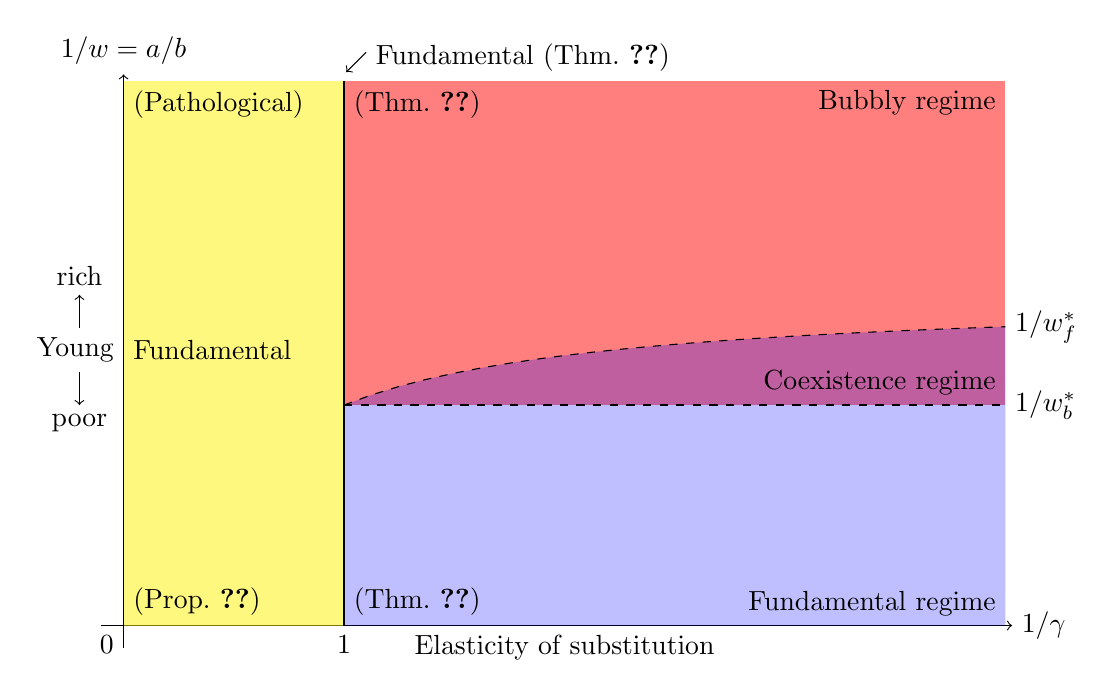
\begin{tikzpicture}[scale = 2.8]

% plot the axes
\draw[->] (-0.1,0) -- (4.03,0) node[right] {$1/\gamma$};
\draw (2,0) node[below] {Elasticity of substitution};
\draw[->] (0,-0.1) -- (0,2.5) node[above] {$1/w=a/b$};
\draw (0,0) node[below left] {$0$};

% fill in color
% pathological region
\fill[semitransparent,yellow] (0,0) rectangle (1,2.47);
\fill[semitransparent,red] (1,1) rectangle (4,2.47); % bubbly region
\fill[nearly transparent,blue,domain = 1:4,variable = \x]
    (1,0)
    -- plot (\x,{1.5^(-1/\x + 1)})
    -- (4,0)
    -- cycle; % fundamental region

% plot boundary for 1/\gamma
\draw (1,0) -- (1,2.47);
\draw (1,0) node[below] {$1$};

% plot boundary for w_f^*
\draw[domain = 1:4,dashed] plot (\x,{1.5^(-1/\x + 1)});
\draw (4,1.355) node[right] {$1/w_f^*$};
% enter G^(-gamma + 1) as y coordinate

% plot boundary for w_b^*
\draw[dashed] (1,1) -- (4,1);
\draw (4,1) node[right] {$1/w_b^*$};

% insert text
% gamma > 1
\draw (0,2.47) node[below right] {(Pathological)};
\draw (0,5/4) node[right] {Fundamental};
\draw (0,0) node[above right] {(Prop.~\ref{prop:gamma>1})};
% gamma = 1
\draw[->] (1.1,2.6) -- (1.01,2.51);
\draw (1.1,2.47) node[above right] {Fundamental (Thm.~\ref{thm:gamma=1})};
% \gamma < 1
\draw (4,0) node[above left] {Fundamental regime};
\draw (1,0) node[above right] {(Thm.~\ref{thm:gamma<1f})};
%\draw[->] (3.8,0.9) -- (3.9,0.9) -- (3.9,1.18);
%\draw (3.8,1) node[below left] {Fundamental \& Bubbly};
\draw (4,1) node[above left] {Coexistence regime};
\draw (4,2.47) node[below left] {Bubbly regime};
\draw (1,2.47) node[below right] {(Thm.~\ref{thm:gamma<1b})};

\draw (0,5/4) node[left] {Young};
\draw[->] (-0.2,1.35) -- (-0.2,1.5) node[above] {rich};
\draw[->] (-0.2,1.15) -- (-0.2,1) node[below] {poor};
    
\end{tikzpicture}

\caption{Phase transition of equilibrium housing price regimes.}\label{fig:regime}

\caption*{\footnotesize Note: $1/w=a/b$ is the young to old income ratio and $w_b^*,w_f^*$ are the thresholds for the bubbly and fundamental regimes defined by \eqref{eq:w*b} and \eqref{eq:w*f}, respectively. The figure corresponds to the CES utility \eqref{eq:CES} with $\beta=1/2$, $\sigma=1$, and $G=1.5$.}

\end{figure}

\begin{figure}[htb!]
\centering

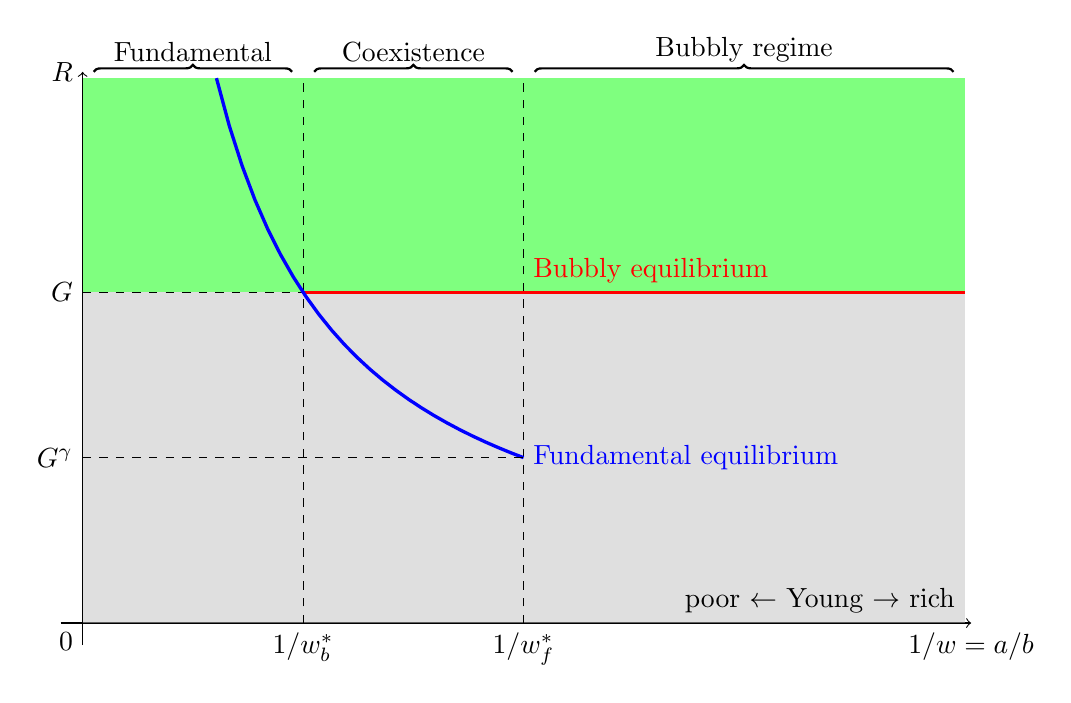
\begin{tikzpicture}[scale = 2.8]

% plot the axes
\draw[->] (-0.1,0) -- (4.03,0) node[below] {$1/w=a/b$};
\draw[->] (0,-0.1) -- (0,2.5) node[left] {$R$};
\draw (0,0) node[below left] {$0$};

% fill in color
% efficient region
\fill[semitransparent,green] (0,1.5) rectangle (4,2.47);
% inefficient region
\fill[semitransparent,lightgray] (0,0) rectangle (4,1.5);

% bubbly equilibrium threshold
\draw[dashed] (1,0) node[below] {$1/w_b^*$} -- (1,2.47);
% fundamental equilibrium threshold
\draw[dashed] (2,0) node[below] {$1/w_f^*$} -- (2,2.47);

%\draw (0,1.5) node[above right] {Efficient};
%\draw (0,1.5) node[below right] {Inefficient};

\draw (4,0) node[above left] {poor $\leftarrow$ Young $\rightarrow$ rich};

% interest rate of bubbly equilibrium
\draw[very thick,red] (1,1.5) -- (4,1.5);
\draw (2,1.5) node[above right,text=red] {Bubbly equilibrium};
\draw[dashed] (0,1.5) -- (1,1.5);
\draw (0,1.5) node[left] {$G$};

% interest rate of fundamental equilibrium
\draw[domain = 0.607:2,very thick,blue] plot (\x,{1.5/\x});
\draw (2,0.75) node[right,text=blue] {Fundamental equilibrium};
\draw[dashed] (0,0.75) -- (2,0.75);
\draw (0,0.75) node[left] {$G^\gamma$};

% Simple brace
\draw [decorate,
    decoration = {brace}, thick] (0.05,2.5) --  (0.95,2.5)
    node[midway,above]{Fundamental};
\draw [decorate,
    decoration = {brace}, thick] (1.05,2.5) --  (1.95,2.5)
    node[midway,above]{Coexistence};
\draw [decorate,
    decoration = {brace}, thick] (2.05,2.5) --  (3.95,2.5)
    node[midway,above]{Bubbly regime};

\end{tikzpicture}
\caption{Housing price regimes and equilibrium interest rate.}\label{fig:interest}
\end{figure}

The intuition for the inevitability of housing bubbles when the young are sufficiently rich is the following. As discussed above, in any fundamental equilibrium, the economy becomes ``house-less'' in the long run, so the long run consumption allocation becomes autarkic. However, as the young get richer (the young to old income ratio $1/w$ increases), the interest rate $R=(c_y/c_z)(1,Gw)$ falls. If $R$ gets lower than a critical value, the economy enters the coexistence regime. Hence, there is a possibility of housing bubbles driven by optimistic expectations. As the income ratio increases further and the fundamental equilibrium interest rate becomes lower than the rent growth rate $G^\gamma$, the only possible equilibrium is one that features a housing bubble. 

\subsection{Long run behavior of housing prices}

We illustrate the preceding analysis with an example. Suppose the composite consumption takes the CES form \eqref{eq:CES}. A straightforward calculation yields
\begin{equation}
    c_y=(1-\beta)(y/c)^{-\sigma} \quad \text{and} \quad c_z=\beta (z/c)^{-\sigma}. \label{eq:CES_grad}
\end{equation}
Using \eqref{eq:w*f}, \eqref{eq:w*b}, and \eqref{eq:CES_grad}, we can solve for the critical values for the existence of fundamental and bubbly equilibria as
\begin{subequations}
\begin{align}
    \frac{1-\beta}{\beta}(Gw_f^*)^\sigma=G^\gamma &\iff w_f^*=\left(\frac{\beta}{1-\beta}G^{\gamma-\sigma}\right)^{1/\sigma}, \label{eq:w*f_CES} \\
    \frac{1-\beta}{\beta}(Gw_b^*)^\sigma=G &\iff w_b^*=\left(\frac{\beta}{1-\beta}G^{1-\sigma}\right)^{1/\sigma}. \label{eq:w*b_CES}
\end{align}
\end{subequations}
Substituting \eqref{eq:CES_grad} into \eqref{eq:s_dynamics2}, we obtain
\begin{equation}
    \beta S_{t+1}z^{-\sigma}=(1-\beta)S_ty^{-\sigma}-m c^{\gamma-\sigma}, \label{eq:s_dynamics_CES}
\end{equation}
where $(y,z)=(a_t-S_t,b_{t+1}+S_{t+1})$. To solve for the equilibrium numerically, we can take a large enough $T$, set $S_T=s^*a_T$ with steady state value $s^*$ defined by
\begin{equation*}
    s^*=\begin{cases*}
        0 & if fundamental equilibrium,\\
        \frac{w_b^*-w}{w_b^*+1} & if bubbly equilibrium,
    \end{cases*}
\end{equation*}
and solve the nonlinear equation \eqref{eq:s_dynamics_CES} backwards for $S_{T-1},\dots,S_0$. Note that the backward calculations of $\set{S_t}_{t=0}^T$ are always possible by Lemma \ref{lem:backward}.

As a numerical example, we set $\beta=1/2$, $\sigma=1$, $\gamma=1/2$, $m=0.1$, and $G=1.1$. The income ratio threshold for the bubbly regime \eqref{eq:w*b_CES} is then $w_b^*=1$. Figure \ref{fig:dynamics_f} shows the equilibrium housing price dynamics when $(a,b)=(95,105)$ so that $b/a>w_b^*$ and hence only a fundamental equilibrium exists. The housing price and rent asymptotically grow at the same rate $G^\gamma$, which is lower than the endowment growth rate $G$. Furthermore, the distance in semilog scale between the housing price and rent converges, suggesting that the price-rent ratio converges. These observations are consistent with Theorem \ref{thm:gamma<1f}.

\begin{figure}[htb!]
    \centering
    \begin{subfigure}{0.48\linewidth}
    \includegraphics[width=\linewidth]{figures/fig_dynamics_f.pdf}
    \caption{Fundamental equilibrium.}\label{fig:dynamics_f}
    \end{subfigure}
    \begin{subfigure}{0.48\linewidth}
    \includegraphics[width=\linewidth]{figures/fig_dynamics_b.pdf}
    \caption{Bubbly equilibrium.}\label{fig:dynamics_b}
    \end{subfigure}
    \caption{Equilibrium housing price dynamics.}\label{fig:dynamics}
\end{figure}

Figure \ref{fig:dynamics_b} repeats the same exercise for $(a,b)=(105,95)$ so that $b/a<w_b^*$ and a bubbly equilibrium exists. The housing price asymptotically grows at the same rate as endowments, while the rent grows at a slower rate. Consequently, the price-rent ratio diverges. These observations are consistent with Theorem \ref{thm:gamma<1b}.

\subsection{Expectation-driven housing bubbles}

We next study how expectations about future incomes affect the current housing price. In Figure \ref{fig:dynamics_fbf_I0}, we consider phase transitions between the fundamental and bubbly regimes. The economy starts with $(a_0,b_0)=(95,105)$ and agents believe that the endowments grow at rate $G$ and the income ratio $b_t/a_t$ is constant at $105/95$. At $t=40$, the income ratio $b_t/a_t$ unexpectedly changes to $95/105$ and agents believe that this new ratio will persist. Thus the economy takes off to the bubbly regime. Finally, at $t=80$ the income ratio $b_t/a_t$ unexpectedly reverts to the original value $105/95$. Note that as the economy enters the bubbly regime, rents are hardly affected but the housing price increases and grows at a faster rate, generating a housing bubble.

\begin{figure}[htb!]
    \centering
    \begin{subfigure}{0.48\linewidth}
    \includegraphics[width=\linewidth]{figures/fig_dynamics_fbf_I0.pdf}
    \caption{Unexpected income change.}\label{fig:dynamics_fbf_I0}
    \end{subfigure}
    \begin{subfigure}{0.48\linewidth}
    \includegraphics[width=\linewidth]{figures/fig_dynamics_fbf_I10.pdf}
    \caption{Expected income change.}\label{fig:dynamics_fbf_I10}
    \end{subfigure}
    \caption{Phase transition between fundamental and bubbly regimes.}\label{fig:dynamics_fbf}
\end{figure}

Figure \ref{fig:dynamics_fbf_I10} repeats the same exercise except that the income changes are anticipated. Specifically, agents learn at $t=30$ that the income ratio will change to $95/105$ (so the young will be relatively rich) starting at $t=40$ and will remain so forever. Similarly, agents learn at $t=70$ that the income ratio will revert to $105/95$ (so the young will be relatively poor) starting at $t=80$ and will remain so forever. In this case, the economy takes off to the bubbly regime at $t=30$ and reenters the fundamental regime at $t=70$ due to rational expectations. We can see that the housing price jumps up at $t=30$ and grows fast even before the fundamentals change. The housing price already contains a bubble, even if the current income of the young is relatively low and appears to be incapable of generating bubbles. This is due to a backward induction argument: if there is a bubble in the future (so \eqref{eq:TVC} holds with strict inequality and the transversality condition fails), there is a bubble in every period. Once the young become relatively rich at $t=40$, the housing price increases at the same rate as endowments, consistent with Theorem \ref{thm:gamma<1b}. During this phase, Irving Fisher would have been right to proclaim that ``prices have reached what looks like a permanently high plateau''.\footnote{\emph{The New York Times}, October 16, 1929, p.~8. URL: \url{https://www.nytimes.com/1929/10/16/archives/fisher-sees-stocks-permanently-high-yale-economist-tells-purchasing.html}.} The housing bubble collapses at $t=70$ when agents learn that the young will be relatively poor in the future, even though the young remain relatively rich until $t=80$. 

From this analysis, we can draw an interesting implication. During expectation-driven housing bubbles, housing prices grow faster than rents. The price-income ratio continues to rise and hence the dynamics may appear unsustainable. Moreover, the greater the time gap between when news of rising incomes arrives ($t=30$) and when incomes actually start to rise ($t=40$), the longer the duration of the seemingly unsustainable dynamics. This expectation-driven housing bubbles and their collapse may capture realistic transitional dynamics.

\section{Welfare}\label{sec:welfare}

In Section \ref{sec:eq}, we saw that housing bubbles emerge as the young get richer. A natural question is whether housing bubbles are socially desirable or not. It is well known that the competitive equilibrium of an overlapping generations model need not be Pareto efficient \citep{Shell1971}. This is because OLG models feature double infinity (infinitely many agents and commodities), which could make the present value of aggregate endowments infinite when the interest rate is low and invalidates the usual proof of the First Welfare Theorem. On the other hand, it is known in the literature since \citet{McCallum1987} that the introduction of fiat money or a non-reproducible asset such as land resolves the over-savings problem in OLG models and eliminates Pareto inefficient equilibria. We overturn this well-known result: even with the presence of non-reproducible housing, Pareto inefficient equilibria can arise. We will show that it crucially depends on the old to young income ratio.

Let $\set{(y_t,z_t,h_t)}_{t=0}^\infty$ be an arbitrary allocation with $y_t,z_t>0$ and $y_t+z_t=a_t+b_t$. Since only the young demand housing service, which is perishable, it is obviously efficient to assign all housing service to the young. Using Assumption \ref{asmp:U}, the utility of generation $t$ becomes
\begin{equation*}
    U(y_t,z_{t+1},1)=u(c(y_t,z_{t+1}))+\phi(1),
\end{equation*}
which is a monotonic transformation of $c(y_t,z_{t+1})$. Therefore the welfare analysis (in terms of Pareto efficiency) reduces to that of an endowment economy without housing and with utility function $c(y,z)$ for goods.

Let $G_t=a_{t+1}/a_t$ be the growth rate of young income and $w_t=b_t/a_t$ be the old to young income ratio at time $t$. Let $s_t=1-y_t/a_t$ be the saving rate. Then the utility of generation $t$ becomes
\begin{equation*}
    c(y_t,z_{t+1})=c(a_t(1-s_t),a_{t+1}(w_{t+1}+s_{t+1}))=a_tc(1-s_t,G_t(w_{t+1}+s_{t+1})),
\end{equation*}
which is a monotonic transformation of $c(1-s_t,G_t(w_{t+1}+s_{t+1}))$. This argument shows that the welfare analysis reduces to the case in which the time $t$ aggregate endowment is $1+w_t$, the utility function of generation $t$ is $u_t(y,z)\coloneqq c(y,G_tz)$, and the proposed allocation is $(y_t,z_t)=(1-s_t,w_t+s_t)$. Since Assumption \ref{asmp:G} implies that $w_t=b_t/a_t$ is constant for $t\ge T$, we can apply the characterization of Pareto efficiency in OLG models with bounded endowments provided by \citet{BalaskoShell1980}. We thus obtain the following proposition.

\begin{prop}[Characterization of equilibrium efficiency]\label{prop:efficient}
Suppose Assumptions \ref{asmp:G}--\ref{asmp:c} hold and an equilibrium $\set{S_t}_{t=0}^\infty$ exists. Let $G_t=a_{t+1}/a_t$, $w_t=b_t/a_t$, and $s_t=S_t/a_t$. Let
\begin{equation}
    R_t=\frac{c_y}{c_z}(1-s_t,G_t(w_{t+1}+s_{t+1})) \label{eq:Rt}
\end{equation}
be the equilibrium risk-free rate and define the Arrow-Debreu price by $q_0=1$ and $q_t=1/\prod_{s=0}^{t-1}R_s$ for $t\ge 1$. Then the following statements are true.
\begin{enumerate}
    \item\label{item:efficient1} If $\liminf_{t\to\infty} R_t>G$, then the equilibrium is Pareto efficient.
    \item\label{item:efficient2} If $\limsup_{t\to\infty}s_t<1$, then the equilibrium is Pareto efficient if and only if
    \begin{equation}
        \sum_{t=0}^\infty \frac{1}{G^tq_t}=\infty. \label{eq:efficient_cond}
    \end{equation}
\end{enumerate}
\end{prop}

Proposition \ref{prop:efficient} is an adaptation of Propositions 5.3 and 5.6 of \citet{BalaskoShell1980} to a growth economy. If we focus on the long run behavior, then $q_t\sim R^{-t}$, so condition \eqref{eq:efficient_cond} implies that the equilibrium is efficient if and only if $R\ge G$. We can now apply Proposition \ref{prop:efficient} to determine whether the equilibria in the housing OLG model are efficient or not.

\begin{thm}[Characterization of equilibrium efficiency]\label{thm:efficient}
Suppose Assumptions \ref{asmp:G}--\ref{asmp:c} hold, $\gamma<1$, and let $w=b/a$. Then the following statements are true.
\begin{enumerate}
    \item If $w\ge w_b^*$, any equilibrium is efficient.
    \item If $w<w_b^*$, any bubbly long run equilibrium is efficient.
    \item If $w<w_b^*$, any fundamental equilibrium is inefficient.
\end{enumerate}
\end{thm}

%Figure \ref{fig:regime} shows how the young to old income ratio $1/w=a/b$ affects the housing price regimes, steady state interest rates, and the efficiency of equilibrium. When the young are poor, the economy is in the fundamental regime and the equilibrium is efficient (because $R>G$). When the income of young exceeds the first threshold, the economy transitions to the coexistence regime, in which the bubbly equilibrium is efficient (because $R=G$) but the fundamental equilibrium is inefficient (because $R<G$). As the young become richer and their income exceeds the second threshold, the economy enters the bubbly regime, in which there exist no fundamental equilibria. The bubbly equilibrium is efficient. By \eqref{eq:R<1f}, the fundamental equilibrium interest rate $R=(c_y/c_z)(1,Gw)$ depends only on $c,G,w$. Therefore in this figure, all elements depend only on $c,G,w$, with the sole exception being the threshold $1/w_f^*$, which also depends on $\gamma$.

Recalling that $w<w_b^*$ implies $R<G$ in the fundamental equilibrium (Figure \ref{fig:interest}), fundamental equilibria are inefficient whenever $R<G$. Therefore in Figure \ref{fig:interest}, all equilibria in the green region (including the boundary) are efficient, whereas all equilibria in the gray region (excluding the boundary) are inefficient.

The intuition for the Pareto inefficiency of fundamental equilibria when $w<w_b^*$ is the following. In equilibrium, since endowments grow at rate $G$ and the elasticity of substitution between consumption and housing is $1/\gamma$, rents grow at rate $G^\gamma$. Therefore if the housing price equals its fundamental value, it must also grow at rate $G^\gamma$. Since $G^\gamma<G$, the housing price is asymptotically negligible relative to endowments, so the equilibrium consumption becomes autarkic. Now when $w<w_b^*$, the young are richer, so the interest rate becomes so low that it is below the economic growth rate (see \eqref{eq:w*b}). In this case if we consider a social contrivance such that for each large enough $t$ the young at time $t$ gives the old $\epsilon G^t$ of the good (hence the old at time $t+1$ receives $\epsilon G^{t+1}$ of the good), it is as if agents are able to save at rate $G$ higher than the interest rate, which improves welfare. Since this argument holds for all large enough $t$, we have a Pareto improvement, which implies the inefficiency of the fundamental equilibrium. 

\section{Discussion}\label{sec:discuss}

\subsection{Testable implications}

Although our paper is theoretical, there are three basic testable implications to be drawn from our analysis. First, from the analysis on the long run behavior, housing bubbles are more likely to emerge if the incomes (or available funds) of home buyers are higher (or expected to be higher). If the incomes of home buyers rise as economic development progresses, housing bubbles may naturally arise first by optimistic expectations, and then inevitably emerge as the optimistic fundamentals materialize. Moreover, our analysis suggests that if the available funds increase with easier access to mortgages, housing bubbles become more likely. Second, if there is a housing bubble on the long run trend, rents grow at rate $G^\gamma$, whereas housing prices grow at rate $G$, implying that the price-rent ratio will rise. Hence, an upward trend in the price-rent ratio could be an indicator for housing bubbles. Third, if the income of home buyers is expected to increase in the future with economic development, this expectation generates a simultaneous rise in the price-rent ratio and the price-income ratio, even before incomes actually start to rise. During this transition, the housing price dynamics may appear unsustainable because prices grow faster than incomes.

\subsection{Related literature}

Our paper belongs to the large literature of rational bubbles. It is well known since \citet{Samuelson1958} and \citet{Tirole1985} that in overlapping generations (OLG) models, a pure bubble asset like fiat money may have a positive price. \citet{Bewley1980} constructed an example with infinitely-lived agents when they are subject to shortsales constraints. \citet{Kocherlakota1992} showed that, in such bubbly equilibria, the present value of endowments must be infinite whenever the shortsales constraint binds. \citet{ArceLopez-Salido2011} and \citet{ChenWen2017} interpret housing bubbles as a situation in which investors purchase vacant housing (pure bubble asset) as a store of value in OLG models with financial frictions. See \citet{Miao2014} and \citet{Guerron-QuintanaHiranoJinnaiAEJ} for the recent development of pure bubble models. The theoretical literature on bubbles has almost exclusively focused on a special case of pure bubbles. Indeed, it is well known that there are fundamental difficulties in generating bubbles in dividend-paying assets summarized by the \citet{SantosWoodford1997} Bubble Impossibility Theorem. A recent paper  by \citet*{HiranoJinnaiTodaBubble} provide the Bubble Characterization Theorem for dividend-paying assets and show that there exist plausible economic models in which a bubbly equilibrium exists but fundamental equilibria do not. They study an endogenous growth model with two sectors, in which in the production sector, heterogeneous entrepreneurs invest capital using leverage and the land sector generates positive dividends. They find that when leverage gets sufficiently high, the production sector grows faster than the land sector, which inevitably makes land prices higher and disconnected from dividends, generating a land price bubble.

Our paper is also related to the literature on the valuation of housing. See \citet{PiazzesiSchneider2016} for a review of the macroeconomic aspect of housing. \citet{MilesMonro2021} emphasize that the decline in the real interest rate has produced large effects on the evolution of housing prices in the U.K. In our model, the (real) interest rate is endogenously determined and is closely related to the income of home buyers. As their income rises and the interest rate falls below the rent growth rate, a housing bubble emerges. \citet{MankiwWeil1989} and \citet*{KiyotakiMichaelidesNikolov2011,KiyotakiMichaelidesNikolov2022}, stress the importance of expectation formation of long run aggregate income growth and the interest rate to account for the fluctuations in housing prices. Our expectation-driven housing bubbles and their collapse show that small changes in fundamentals or the expectation thereof could produce large swings in housing prices.

Concerning the efficiency of OLG economies, it is well known that the over-savings problem (dynamic inefficiency) can arise. However, it is also well known since \citet{McCallum1987} that the existence of a non-reproducible asset like land restores dynamic efficiency. In our model, housing is a non-reproducible asset but the fundamental equilibrium is inefficient whenever the interest rate is lower than the rent growth rate, so we overturn this result.

\subsection{Concluding remarks}

This paper developed a simple overlapping generations model with consumption and housing and identified conditions under which housing bubbles are possible or even inevitable. We offer three key insights. The first is the two-stage phase transition. Whether housing bubbles emerge in equilibrium depends on the long run income ratio between the home buyers and sellers. When the income ratio of the home buyers is sufficiently low, housing bubbles cannot arise and only the fundamental equilibrium exists. When the ratio rises and exceeds the first critical value, a phase transition occurs. Both fundamental and bubbly equilibria exist, and agents' expectations play a key role in determining the long run path of the economy. This also implies that even if there is no substantial change in fundamentals, housing bubbles can burst depending on agents' beliefs. If the income ratio exceeds the second and still higher critical value, another phase transition takes place. The only possible equilibrium is one that features housing bubbles. In other words, bubbles are inevitable for the existence of equilibrium.

The second insight is the expectation-driven housing bubbles. Because agents are forward-looking and housing prices reflect information about the states of the future economy, whether bubbles arise or not in equilibrium depends on long run expectations about the income ratio of home buyers. Even if the current income of home buyers is low, as long as agents expect high incomes in the future, housing prices start rising now and contain a bubble, even if the current fundamentals do not change and may appear incapable of generating a bubble. On the other hand, if these optimistic expectations do not materialize, the bubble will collapse.

The third insight is the welfare implications. It has been widely believed in the literature that the introduction of a productive non-reproducible asset like land eliminates the dynamic inefficiency in overlapping generations model. We showed that this is not necessarily true: inefficient equilibria can still occur. In the region where fundamental and bubbly equilibria coexist, the bubbly equilibrium is efficient but the fundamental equilibrium is not. Therefore policymakers may have a role in guiding expectations and equilibrium selection.

\appendix

\section{Proofs}\label{sec:proof}

\subsection{Proof of Section \ref{sec:eq} results}

 The following lemma lists a few implications of Assumption \ref{asmp:c} that will be repeatedly used.

\begin{lem}\label{lem:c}
Suppose Assumption \ref{asmp:c} holds and let $g(x)\coloneqq c(x,1)$. Then the following statements are true.
\begin{enumerate}
    \item The first partial derivatives of $c$ are given by
    \begin{subequations}\label{eq:c_partial1}
    \begin{align}
        c_y(y,z)&=g'(y/z)>0,\\
        c_z(y,z)&=g(y/z)-(y/z)g'(y/z)>0
    \end{align}
    \end{subequations}
    and are homogeneous of degree 0.
    \item The second partial derivatives are given by
    \begin{subequations}\label{eq:c_partial2}
    \begin{align}
        c_{yy}(y,z)&=\frac{1}{z}g''(y/z)<0, \\
        c_{yz}(y,z)&=-\frac{y}{z^2}g''(y/z)>0, \\
        c_{zz}(y,z)&=\frac{y^2}{z^3}g''(y/z)<0.
    \end{align}
    \end{subequations}
    \item Fixing $z>0$, the marginal rate of substitution $c_y/c_z$ is continuously differentiable and strictly decreasing in $y$ and has range $(0,\infty)$.
    \item The elasticity of intertemporal substitution is $\varepsilon(y,z)=\frac{c_yc_z}{cc_{yz}}>0$.
\end{enumerate}
\end{lem}

\begin{proof}%[Proof of Lemma \ref{lem:c}]
By definition, $g(x)=c(x,1)$. Therefore $g'(x)=c_y(x,1)>0$ and $g''(x)=c_{yy}(x,1)<0$ by Assumption \ref{asmp:c}. Since $c$ is homogeneous of degree 1, we have $c(y,z)=zc(y/z,1)=zg(y/z)$. Then \eqref{eq:c_partial1} and \eqref{eq:c_partial2} are immediate by direct calculation.

Fixing $z>0$, define the marginal rate of substitution $M(y)=(c_y/c_z)(y,z)$. Then $M$ is continuously differentiable because $c$ is twice continuously differentiable and $c_y,c_z>0$. Since $c_y,c_z$ are homogeneous of degree 0, we have
\begin{equation}
    M(y)=\frac{c_y(y,z)}{c_z(y,z)}=\frac{c_y(y/z,1)}{c_z(1,z/y)}. \label{eq:My}
\end{equation}
Since $c_y,c_z>0$ and $c_{yy},c_{zz}<0$, the numerator (denominator) is positive and strictly decreasing (increasing) in $y$. Therefore $M$ is strictly decreasing. Furthermore, since $c_y(0,z)=c_z(y,0)=\infty$, letting $y\downarrow 0$ and $y\uparrow \infty$ in \eqref{eq:My}, we obtain $M(0)=\infty$ and $M(\infty)=0$, so $M$ has range $(0,\infty)$.

Finally, we derive the elasticity of intertemporal substitution (EIS) $\varepsilon$. Since $c$ is homogeneous of degree 1, we have $c(\lambda y,\lambda z)=\lambda c(y,z)$. Differentiating both sides with respect to $\lambda$ and setting $\lambda=1$, we obtain
\begin{equation}
    yc_y+zc_z=c.\label{eq:c_Euler}
\end{equation}
Letting $\sigma=1/\varepsilon$ and $x=y/z$, by the chain rule we obtain
\begin{align*}
    \sigma&=-\frac{\partial \log (c_y/c_z)(xz,z)}{\partial \log x}=-x\frac{c_z}{c_y}\frac{zc_{yy}c_z-c_yzc_{yz}}{c_z^2}\\
    &=y\frac{c_yc_{yz}-c_zc_{yy}}{c_yc_z}=\frac{(yc_y+zc_z)c_{yz}}{c_yc_z}=\frac{cc_{yz}}{c_yc_z},
\end{align*}
where the last line uses \eqref{eq:c_partial2} and \eqref{eq:c_Euler}.
\end{proof}

\begin{proof}[Proof of Lemma \ref{lem:backward}]
Suppose an equilibrium $\cS_T=\set{S_t}_{t=T}^\infty$ starting at $t=T$ exists. Set $t=T-1$ and define the function $f:[0,a_{T-1})\to \R$ by
\begin{equation*}
    f(S)=S_Tc_z-Sc_y+mc^\gamma,
\end{equation*}
where $c,c_y,c_z$ are evaluated at $(y,z)=(a_{T-1}-S,b_T+S_T)$. Then
\begin{equation*}
    f'(S)=-S_Tc_{yz}-c_y+Sc_{yy}-m\gamma c^{\gamma-1}c_y<0
\end{equation*}
by Lemma \ref{lem:c}. Clearly $f(0)=S_Tc_z+mc^\gamma>0$. Define
\begin{equation}
    v(y,z)\coloneqq u(c(y,z))=\begin{cases*}
        \frac{1}{1-\gamma}c(y,z)^{1-\gamma} & if $\gamma\neq 1$,\\
        \log(c(y,z)) & if $\gamma=1$.
    \end{cases*}\label{eq:vyz}
\end{equation}
Take any $\bar{y}>0$ and let $0<y<\bar{y}$. Using the chain rule and the monotonicity of $c$, we obtain
\begin{equation}
    v_y(y,z)=c(y,z)^{-\gamma}c_y(y,z)>c(\bar{y},z)^{-\gamma}c_y(y,z)\to \infty \label{eq:v_Inada}
\end{equation}
as $y\downarrow 0$ by Assumption \ref{asmp:c}. Using the definition of $f$, we obtain $f(S)c^{-\gamma}=S_Tv_z-Sv_y+m$.
Letting $S\uparrow a_{T-1}$ and using \eqref{eq:v_Inada}, we obtain $f(S)c^{-\gamma}\to -\infty$. Hence by the intermediate value theorem, there exists a unique $S_{T-1}\in (0,a_{T-1})$ such that $f(S_{T-1})=0$. Therefore there exists a unique equilibrium $\cS_{T-1}=\set{S_t}_{t=T-1}^\infty$ starting at $t=T-1$ that agrees with $\cS_T$ for $t\ge T$. The claim follows from backward induction.
\end{proof}

\begin{proof}[Proof of Lemma \ref{lem:r_bound}]
Take any equilibrium. Using \eqref{eq:eq_r} and Assumption \ref{asmp:U}, the rent is
\begin{equation}
    r_t=m\frac{c^\gamma}{c_y}(aG^t-S_t,bG^{t+1}+S_{t+1}). \label{eq:r_explicit}
\end{equation}
Using the trivial bound $0\le S_t\le aG^t$, noting that $c$ is increasing in both arguments and $c_y$ is decreasing (increasing) in $y$ ($z$) by Lemma \ref{lem:c}, and using the homogeneity of $c$ and $c_y$, we obtain
\begin{equation*}
    r_t\le m\frac{c(aG^t,(a+b)G^{t+1})^\gamma}{c_y(aG^t,bG^{t+1})}=ma^\gamma\frac{c(1,G(1+w))}{c_y(1,Gw)}G^{\gamma t}\eqqcolon \bar{r}G^{\gamma t}.
\end{equation*}

Next, suppose that $\limsup_{t\to\infty}S_t/a_t<1$. Since $S_t<a_t$ (because young consumption $y_t=a_t-S_t$ must be positive by the Inada condition), we can take $\bar{s}<1$ such that $S_t/a_t\le \bar{s}$ for all $t$. Then by a similar argument, we obtain
\begin{equation*}
    r_t\ge m\frac{c((a-a\bar{s})G^t,bG^{t+1})^\gamma}{c_y((a-a\bar{s})G^t,(a+b)G^{t+1})}=ma^\gamma\frac{c(1-\bar{s},Gw)}{c_y(1-\bar{s},G(1+w))}\eqqcolon \ubar{r}G^{\gamma t}. \qedhere
\end{equation*}
\end{proof}

To prove Theorem \ref{thm:gamma<1f}, we establish a series of lemmas. In the discussion below, we suppose that Assumptions \ref{asmp:G}--\ref{asmp:c} hold and $\gamma<1$. Note that by Proposition \ref{prop:eq}, the equilibrium is fully characterized by the sequence of housing expenditure $\set{S_t}_{t=0}^\infty$.

\begin{lem}\label{lem:w*f}
There exists a unique $w_f^*>0$ satisfying \eqref{eq:w*f}.
\end{lem}

\begin{proof}
By Lemma \ref{lem:c}, $(c_y/c_z)(v,G)$ is strictly decreasing in $v$ and has range $(0,\infty)$. Therefore there exists a unique $v$ satisfying $(c_y/c_z)(v,G)=G^\gamma$. Since by Lemma \ref{lem:c} $c_y,c_z$ are homogeneous of degree 0, we have $(c_y/c_z)(1,G/v)=G^\gamma$, so $w_f^*=1/v$ uniquely satisfies \eqref{eq:w*f}.
\end{proof}

\begin{lem}\label{lem:f_order}
    In any fundamental equilibrium, the equilibrium objects have the order of magnitude in \eqref{eq:eqobj_gamma<1f}.
\end{lem}

\begin{proof}
\setcounter{step}{0}
Let $\set{S_t}_{t=0}^\infty$ be a fundamental equilibrium. We divide the proof into several steps.

\begin{step}
    If $\limsup_{t\to\infty}G^{-t}S_t>0$, then $\liminf_{t\to\infty}R_t\ge G$.
\end{step}

Using the upper bound $S_t\le \bar{r}G^{\gamma t}$ in Lemma \ref{lem:r_bound} and $\gamma<1$, we obtain
\begin{equation}
    \limsup_{t\to\infty}G^{-t}P_t=\limsup_{t\to\infty}G^{-t}(S_t-r_t)=\limsup_{t\to\infty}G^{-t}S_t>0. \label{eq:limsup}
\end{equation}
Suppose to the contrary that $\liminf_{t\to\infty}R_t<G$. Then we can take $T>0$ such that $R_t\le G$ for $t\ge T$. Letting $q_t>0$ be the Arrow-Debreu price, it follows that
\begin{equation*}
    q_tP_t=\left(q_T\prod_{s=T}^{t-1}\frac{1}{R_s}\right)P_t\ge q_T G^{T-t}P_t=q_TG^TG^{-t}P_t.
\end{equation*}
Letting $t\to\infty$, it follows from \eqref{eq:limsup} that $\limsup_{t\to\infty}q_tP_t>0$, which contradicts the transversality condition that must hold in fundamental equilibria.

\begin{step}
    $\lim_{t\to\infty}G^{-t}S_t=0$.
\end{step}

Suppose to the contrary that $\limsup_{t\to\infty}G^{-t}S_t>0$. Then by the previous step, we have $\liminf_{t\to\infty}R_t\ge G>G^\gamma$. Take $R\in (G^\gamma,G)$. Then we can take $T>0$ such that $R_t\ge R$ for $t\ge T$. Since by assumption the equilibrium housing price equals its fundamental value (present value of rents), using Lemma \ref{lem:r_bound}, for $t\ge T$ we can bound the housing price from above as
\begin{equation}
    P_t\le \bar{r}G^{\gamma t}\sum_{s=1}^\infty (G^\gamma/R)^s=\bar{r}G^{\gamma t}\frac{G^\gamma}{R-G^\gamma}. \label{eq:P_ub}
\end{equation}
Since both $r_t$ and $P_t$ grow at rate at most $G^\gamma<G$ by Lemma \ref{lem:r_bound} and \eqref{eq:P_ub}, so does $S_t=P_t+r_t$. Therefore $\lim_{t\to\infty}G^{-t}S_t=0$, which contradicts the assumption.

\begin{step}
    The equilibrium objects have the order of magnitude in \eqref{eq:eqobj_gamma<1f} and the housing price equals its fundamental value.
\end{step}

The order of magnitude \eqref{eq:eqobj_gamma<1f} is obvious from $\lim_{t\to\infty}G^{-t}S_t=0$, the homogeneity of $c$, and Proposition \ref{prop:eq}. In equilibrium, the housing price $P_t$ asymptotically grows at rate $G^\gamma$. Since by \eqref{eq:R<1f} the interest rate eventually exceeds the growth rate of the housing price, the transversality condition
\begin{equation*}
    \lim_{T\to\infty} \left(\prod_{t=0}^{T-1}R_t\right)^{-1}P_T=0
\end{equation*}
holds and the housing price equals its fundamental value.
\end{proof}

\begin{lem}\label{lem:nonexist}
    If $w<w_f^*$, there exist no fundamental equilibria.
\end{lem}

\begin{proof}
Suppose a fundamental equilibrium exists. Then by \eqref{eq:R<1f}, Lemma \ref{lem:c}, and $w<w_f^*$, we obtain
\begin{equation}
R_t\to (c_y/c_z)(1,Gw)<(c_y/c_z)(1,Gw_f^*)=G^\gamma. \label{eq:Rt_lim}
\end{equation}
Since by \eqref{eq:r<1f} the rent asymptotically grows at rate $G^\gamma$, which exceeds the asymptotic interest rate by \eqref{eq:Rt_lim}, the present value of rents is infinite, which is impossible in equilibrium.
\end{proof}

\begin{proof}[Proof of Theorem \ref{thm:gamma<1f}]
The proofs of all results except existence follow from Lemmas \ref{lem:w*f}--\ref{lem:nonexist}. We divide the existence proof into several steps.

\setcounter{step}{0}

\begin{step}
    Derivation of an autonomous nonlinear difference equation.
\end{step}

By \eqref{eq:p<1f} and \eqref{eq:r<1f}, if a fundamental equilibrium exists, $S_t=P_t+r_t$ asymptotically grow at rate $G^\gamma$. Define the detrended variable $s_t\coloneqq S_t/(a^\gamma G^{\gamma t})$. Using the homogeneity of $c,c_y,c_z$, \eqref{eq:s_dynamics2} implies
\begin{equation}
    a^\gamma s_{t+1}G^{\gamma(t+1)}c_z-a^\gamma s_tG^{\gamma t}c_y+ma^\gamma G^{\gamma t}c^\gamma, \label{eq:s_dynamics5}
\end{equation}
where $c,c_y,c_z$ are evaluated at
\begin{equation*}
    (y,z)=(1-s_ta^{\gamma-1}G^{(\gamma-1)t},G(w+s_{t+1}a^{\gamma-1}G^{(\gamma-1)(t+1)})).
\end{equation*}
Dividing \eqref{eq:s_dynamics5} by $a^\gamma G^{\gamma t}$ and defining the auxiliary variable $\xi_t=(\xi_{1t},\xi_{2t})=(s_t,a^{\gamma-1}G^{(\gamma-1)t})$, it follows that \eqref{eq:s_dynamics2} can be rewritten as $H(\xi_t,\xi_{t+1})=0$, where $H:\R^4\to \R^2$ is given by
\begin{subequations}\label{eq:H2}
    \begin{align}
        H_1(\xi,\eta)&=G^\gamma\eta_1c_z-\xi_1 c_y+mc^\gamma,\\
        H_2(\xi,\eta)&=\eta_2-G^{\gamma-1}\xi_2
    \end{align}
\end{subequations}
and $c,c_y,c_z$ are evaluated at
\begin{equation*}
    (y,z)=(1-\xi_{1t}\xi_{2t},G(w+\xi_{1,t+1}\xi_{2,t+1})).
\end{equation*}


\begin{step}
    Existence and uniqueness of a fundamental steady state.
\end{step}



If a steady state $\xi_f^*$ of \eqref{eq:H2} exists, it must be $\xi_2=0$. Then the steady state condition is
\begin{equation*}
    G^\gamma sc_z-sc_y+mc^\gamma\iff s=m\frac{c^\gamma}{c_y-G^\gamma c_z},
\end{equation*}
where $c,c_y,c_z$ are evaluated at $(y,z)=(1,Gw)$. For $s>0$, it is necessary and sufficient that $c_y/c_z>G^\gamma$ at $(y,z)=(1,Gw)$. Since by Lemma \ref{lem:c} $c_y,c_z$ are homogeneous of degree 0 and $c_y/c_z$ is strictly increasing in $z$, there exists a fundamental steady state if and only if $w>w_f^*$.

\begin{step}
    Existence and local determinacy of equilibrium.
\end{step}

Define $H$ by \eqref{eq:H2} and write $s=s^*$ to simplify notation. Noting that $\xi_f^*=(s^*,0)$, a straightforward calculation yields
\begin{align*}
    D_\xi H(\xi_f^*,\xi_f^*)&=\begin{bmatrix}
        -c_y & -G^\gamma s^2c_{yz}+s^2c_{yy}-sm\gamma c^{\gamma-1}c_y\\
        0 & -G^{\gamma-1}
    \end{bmatrix},\\
    D_\eta H(\xi_f^*,\xi_f^*)&=\begin{bmatrix}
        G^\gamma c_z & G^{\gamma+1}s^2c_{zz}-Gs^2c_{yz}+Gsm\gamma c^{\gamma-1}c_z\\
        0 & 1
    \end{bmatrix},
\end{align*}
where all functions are evaluated at $(y,z)=(1,Gw)$. Since $D_\eta H$ is invertible, we may apply the implicit function theorem to solve $H(\xi,\eta)=0$ around $(\xi,\eta)=(\xi_f^*,\xi_f^*)$ as $\eta=h(\xi)$, where
\begin{equation*}
    Dh(\xi_f^*)=-[D_\eta H]^{-1}D_\xi H=\begin{bmatrix}
        \frac{c_y}{G^\gamma c_z} & h_{12}\\
        0 & G^{\gamma-1}
    \end{bmatrix}
\end{equation*}
and $h_{12}$ is unimportant. Since $c_y>G^\gamma c_z$, the eigenvalues of $Dh$ are $\lambda_1=c_y/(G^\gamma c_z)>1$ and $\lambda_2=G^{\gamma-1}\in (0,1)$. Therefore the steady state $\xi_f^*$ is a saddle point. The local stable manifold theorem (see \citet[Theorems 6.5 and 6.9]{Irwin1980} and \citet[Theorem 1.4.2]{GuckenheimerHolmes1983}) implies that for any sufficiently large $a>0$ (so that $\xi_{20}=a^{\gamma-1}$ is close to the steady state value 0), there exists a unique orbit $\set{\xi_t}_{t=0}^\infty$ converging to the steady state $\xi_f^*$. However, by Assumption \ref{asmp:G}, choosing a large enough $a>0$ is equivalent to starting the economy at large enough $t=T$. Lemma \ref{lem:backward} then implies that there exists a unique equilibrium converging to the steady state regardless of the early endowments $\set{(a_t,b_t)}_{t=0}^{T-1}$.
\end{proof}

\begin{proof}[Proof of Theorem \ref{thm:gamma<1b}]
We divide the proof into several steps.

\setcounter{step}{0}

\begin{step}
    Existence and uniqueness of a bubbly steady state.
\end{step}

The proof of the existence and uniqueness of $w_b^*$ satysfing \eqref{eq:w*b} is identical to Lemma \ref{lem:w*f}. Since $G>1$ and $\gamma<1$, it follows from \eqref{eq:w*f} and \eqref{eq:w*b} that
\begin{equation*}
    (c_y/c_z)(1,Gw_f^*)=G^\gamma<G=(c_y/c_z)(1,Gw_b^*).
\end{equation*}
Since by Lemma \ref{lem:c} $c_y/c_z$ is strictly decreasing in $y$ (and hence strictly increasing in $z$), we obtain $w_f^*<w_b^*$.

The steady state condition is $Gc_z-c_y=0$, where $c_y,c_z$ are evaluated at $(y,z)=(1-s,G(w+s))$. Using the homogeneity of $c_y,c_z$, this condition is equivalent to $(c_y/c_z)(v,G)=G$ for $v=\frac{1-s}{w+s}$, so the bubbly steady state is uniquely determined by
\begin{equation}
    \frac{1-s}{w+s}=\frac{1}{w_b^*}\iff s=\frac{w_b^*-w}{w_b^*+1}. \label{eq:s*<1}
\end{equation}
Since $s\in (0,1)$, a necessary and sufficient condition for the existence of a bubbly steady state is $w<w_b^*$.

\begin{step}
    Order of magnitude of equilibrium objects and asset pricing implications.
\end{step}

In any equilibrium converging to the bubbly steady state, by definition we have $S_t\sim asG^t$, where $s=s^*$ is the bubbly steady state. Therefore \eqref{eq:yz<1b} follows from \eqref{eq:eq_yz}. Using \eqref{eq:eq_r} and Assumption \ref{asmp:U}, the rent is
\begin{equation}
    r_t=\frac{\phi'(1)}{u'(c)c_y}=m\frac{c(a_t-S_t,b_{t+1}+s_{t+1})^\gamma}{c_y(a_t-S_t,b_{t+1}+s_{t+1})}.\label{eq:r_gamma}
\end{equation}
Substituting \eqref{eq:yz<1b} into \eqref{eq:r_gamma} and using the fact that $c$ is homogeneous of degree 1 and $c_y$ is homogeneous of degree 0, we obtain
\begin{equation*}
    r_t\sim ma^\gamma \frac{c(1-s,G(w+s))^\gamma}{c_y(1-s,G(w+s))}G^{\gamma t},
\end{equation*}
which is \eqref{eq:r<1b}. Since $r_t$ asymptotically grows at rate $G^\gamma<G$ because $\gamma<1$, we have $r_t/S_t\to 0$, so $P_t=S_t-r_t\sim S_t$, which is \eqref{eq:p<1b}. Finally, \eqref{eq:R<1b} follows from \eqref{eq:R}, \eqref{eq:p<1b}, and \eqref{eq:r<1b}.

Since the housing price $S_t$ and rent $r_t$ asymptotically grow at rates $G$ and $G^\gamma<G$, respectively, the price-rent ratio $S_t/r_t$ asymptotically grows at rate $G^{1-\gamma}>1$ and diverges to infinity. Since the gross risk-free rate \eqref{eq:R<1b} converges to $G$ and the rent grows at rate $G^\gamma<G$, the present value of rents is finite and so is the fundamental value of housing. However, because $S_t\to\infty$, the housing price eventually exceeds the fundamental value. Therefore the transversality condition fails and there is a housing bubble.

\begin{step}
    Generic existence of equilibrium.
\end{step}

Define $H$ by \eqref{eq:H} and write $s=s^*$ to simplify notation. Noting that $\xi_b^*=(s^*,0)$, a straightforward calculation yields
\begin{align*}
    D_\xi H(\xi_b^*,\xi_b^*)&=\begin{bmatrix}
        -Gs c_{yz}-c_y+sc_{yy} & mc^\gamma \\
        0 & -G^{\gamma-1}
    \end{bmatrix},\\
    D_\eta H(\xi_b^*,\xi_b^*)&=\begin{bmatrix}
        Gc_z+G^2s c_{zz}-Gsc_{yz} & 0\\
        0 & 1
    \end{bmatrix},
\end{align*}
where all functions are evaluated at $(y,z)=(1-s,G(w+s))$. If $D_\eta H$ is invertible, we may apply the implicit function theorem to solve $H(\xi,\eta)=0$ around $(\xi,\eta)=(\xi_b^*,\xi_b^*)$ as $\eta=h(\xi)$, where
\begin{equation*}
    Dh(\xi_b^*)=-[D_\eta H]^{-1}D_\xi H=\begin{bmatrix}
        h_{11} & h_{12}\\
        0 & G^{\gamma-1}
    \end{bmatrix}
\end{equation*}
with
\begin{equation}
    h_{11}=\frac{Gs c_{yz}+c_y-sc_{yy}}{Gc_z+G^2s c_{zz}-Gsc_{yz}}\eqqcolon \frac{e}{d} \label{eq:h11}
\end{equation}
and $h_{12}$ is unimportant.  Therefore $Dh(\xi_b^*)$ has two real eigenvalues; one is $\lambda_1\coloneqq h_{11}$ and the other is $\lambda_2 \coloneqq G^{\gamma-1}\in (0,1)$ because $G>1$ and $\gamma\in (0,1)$.

Let us estimate $\lambda_1$. Using \eqref{eq:c_partial2}, the numerator of \eqref{eq:h11} is
\begin{align*}
    e&=c_y+s(Gc_{yz}-c_{yy})=c_y+s\left(-G\frac{y}{z^2}g''-\frac{1}{z}g''\right)\\
    &=c_y-s\frac{Gy+z}{z^2}g''=c_y-\frac{s(1+w)}{G(w+s)^2}g'',
\end{align*}
where we have used $(y,z)=(1-s,G(w+s))$. Similarly, the denominator is
\begin{align*}
    d&=Gc_z+Gs(Gc_{zz}-c_{yz})=Gc_z+Gs\left(G\frac{y^2}{z^3}g''+\frac{y}{z^2}g''\right)\\
    &=Gc_z+Gs\frac{y(Gy+z)}{z^3}g''=Gc_z+\frac{s(1-s)(1+w)}{G(w+s)^3}g''.
\end{align*}
At the steady state, we have $Gc_z=c_y=g'$, so
\begin{subequations}\label{eq:ed}
    \begin{align}
        e&=g'-\frac{s(1+w)}{G(w+s)^2}g'',\\
        d&=g'+\frac{s(1-s)(1+w)}{G(w+s)^3}g''.
    \end{align}
\end{subequations}
Since $s\in (0,1)$ and $g''<0$, clearly $e>d$.

We now study each case by the magnitude of $d$.

\begin{case}[$d>0$]
If $d>0$, then $0<d<e$ and hence $\lambda_1=e/d>1$. Since $\lambda_1>1>\lambda_2>0$, the steady state $\xi_b^*$ is a saddle point. The existence and uniqueness of an equilibrium path converging to the steady state $\xi_b^*$ follows by the same argument as in the proof of Theorem \ref{thm:gamma<1f}.
\end{case}
\begin{case}[$d=0$]
If $d=0$, the implicit function theorem is inapplicable and we cannot study the local dynamics by linearization.
\end{case}
\begin{case}[$d\in (-e,0)$]
If $-e<d<0$, then $\lambda_1=e/d<-1$. Therefore $\xi_b^*$ is a saddle point and there exists a unique equilibrium by the same argument as in the case $d>0$.
\end{case}
\begin{case}[$d=-e$]
If $d=-e$, then $\lambda_1=e/d=-1$ and the local stable manifold theorem is inapplicable.
\end{case}
\begin{case}[$d<-e$]
If $d<-e$, then $\lambda_1=e/d\in (-1,0)$. Therefore $\xi_b^*$ is a sink and there exist a continuum of equilibria by the same argument as in the case $d>0$.
\end{case}
In summary, there exists an equilibrium converging to the bubbly steady state except when $d=0$ or $d=-e$. Therefore for generic $G$ and $w$, there exists an equilibrium.
\end{proof}

\begin{proof}[Proof of Proposition \ref{prop:unique}]
We have already proved the uniqueness of the fundamental equilibrium if $w>w_f^*$ in the proof of Theorem \ref{thm:gamma<1f}.

Suppose $w<w_b^*$. Let $s=\frac{w_b^*-w}{w_b^*+1}$ be the bubbly steady state and $(y,z)=(1-s,G(w+s))$. By the proof of Theorem \ref{thm:gamma<1b}, there exists a unique equilibrium converging to the bubbly steady state if $d\in (-e,0)\cup (0,\infty)$, where $d,e$ are as in \eqref{eq:ed}. We rewrite this condition using the EIS defined by $\varepsilon=\frac{c_yc_z}{cc_{yz}}$. Using \eqref{eq:c_partial1}, \eqref{eq:c_partial2}, \eqref{eq:c_Euler}, and $Gc_z=c_y$ at the steady state, we obtain
\begin{equation*}
    \varepsilon=\frac{c_yc_z}{(yc_y+zc_z)c_{yz}}=\frac{c_y}{(Gy+z)c_{yz}}=-\frac{g'}{g''}\frac{G(w+s)^2}{(1-s)(1+w)}.
\end{equation*}
Therefore \eqref{eq:ed} can be rewritten as
\begin{subequations}\label{eq:ed2}
    \begin{align}
        e&=\left(1+\frac{1}{\varepsilon}\frac{s}{1-s}\right)g',\\
        d&=\left(1-\frac{1}{\varepsilon}\frac{s}{w+s}\right)g'.
    \end{align}
\end{subequations}
Since $g'>0$, we have
\begin{align*}
    d=0&\iff \varepsilon=\frac{s}{w+s}=\frac{1-w/w_b^*}{1+w},\\
    e+d>0&\iff \varepsilon>\frac{s(1-w-2s)}{2(1-s)(w+s)}=\frac{1-w_b^*}{2}\frac{1-w/w_b^*}{1+w}.
\end{align*}
Therefore the sufficient condition \eqref{eq:locdet_gamma<1} follows.
\end{proof}

\subsection{Proof of Section \ref{sec:welfare} results}

\begin{proof}[Proof of Proposition \ref{prop:efficient}]
Let $u_t(y,z)=c(y,G_tz)$ be the utility function in the detrended economy. Then the implied gross risk-free rate at the proposed allocation $(y_t,z_{t+1})=(1-s_t,w_{t+1}+s_{t+1})$ is
\begin{equation*}
    \tilde{R}_t\coloneqq \frac{u_{ty}}{u_{tz}}(1-s_t,w_{t+1}+s_{t+1})=\frac{1}{G_t}\frac{c_y}{c_z}(1-s_t,w_{t+1}+s_{t+1})=\frac{R_t}{G_t}.
\end{equation*}
Therefore the Arrow-Debreu price in the detrended economy is $\tilde{q}_t=\prod_{s=0}^{t-1}(G_s/R_s)$.

We now apply the results of \citet{BalaskoShell1980}. If $\liminf_{t\to\infty}R_t>G$, then by Assumption \ref{asmp:G} we can take $R>G$ such that $R_t\ge R>G=G_t$ for $t$ large enough. Then $G_t/R_t\le G/R<1$, so we have $\lim_{t\to\infty} \tilde{q}_t=0$. Proposition 5.3 of \citet{BalaskoShell1980} then implies that the equilibrium is efficient.

We next consider the case $\bar{s}\coloneqq \limsup_{t\to\infty}s_t<1$. We verify each assumption of Proposition 5.6 of \citet{BalaskoShell1980}. Since the partial derivatives of $c$ can be signed as in Lemma \ref{lem:c}, the Gaussian curvature of indifference curves are strictly positive. Since the time $t$ aggregate endowment of the detrended economy is $1+w_t$, which is bounded by Assumption \ref{asmp:G}, it follows that the Gaussian curvature of indifference curves within the feasible region (weakly preferred to endowments) is uniformly bounded and bounded away from 0 because $1-\bar{s}>0$. Therefore assumptions (a) and (b) hold. Since $\bar{s}<1$ and $G_t$, $w_{t+1}$ are bounded, the gross risk-free rate \eqref{eq:Rt} can be uniformly bounded from above and away from 0. Therefore assumption (c) holds. Assumption (d) holds because $w_t$ is bounded, and assumption (e) holds because $\liminf_{t\to\infty}(1-s_t)=1-\bar{s}>0$. Since all assumptions are verified, Proposition 5.6 of \citet{BalaskoShell1980} implies that the equilibrium is efficient if and only if
\begin{equation}
    \infty=\sum_{t=0}^\infty \frac{1}{\tilde{q}_t}=\sum_{t=0}^\infty \frac{1}{q_t\prod_{s=0}^{t-1}G_s}.\label{eq:BS_cond}
\end{equation}
Since by Assumption \ref{asmp:G} we have $G_t=G$ for large enough $t$, \eqref{eq:BS_cond} is clearly equivalent to \eqref{eq:efficient_cond}.
\end{proof}

\begin{proof}[Proof of Theorem \ref{thm:efficient}]
Suppose $\gamma<1$ and consider any equilibrium. Using \eqref{eq:Rt}, Assumption \ref{asmp:G}, Lemma \ref{lem:c}, and $s_t\ge 0$, we obtain
\begin{equation}
    R_t=\frac{c_y}{c_z}(1-s_t,G_t(w_{t+1}+s_{t+1}))\ge \frac{c_y}{c_z}(1,Gw) \label{eq:Rt_lb}
\end{equation}
for large enough $t$. If $w\ge w_b^*$, then \eqref{eq:Rt_lb}, Lemma \ref{lem:c}, and \eqref{eq:w*b} imply
\begin{equation*}
    R_t\ge \frac{c_y}{c_z}(1,Gw)\ge \frac{c_y}{c_z}(1,Gw_b^*)=G.
\end{equation*}
Since $R_t\ge G$ eventually, the sequence $1/(G^tq_t)=\prod_{s=0}^{t-1}(R_s/G)$ is positive and bounded away from 0. Therefore \eqref{eq:efficient_cond} holds, and the equilibrium is efficient.

Suppose $w<w_b^*$ and take any bubbly equilibrium converging to the bubbly steady state. By \eqref{eq:p<1b}, we can take $p>0$ such that $P_t\ge pG^t$ for large enough $t$. Then
\begin{equation*}
    G^tq_t=\frac{1}{p}q_tpG^t\le \frac{1}{p}q_tP_t\le \frac{1}{p}P_0
\end{equation*}
using \eqref{eq:P_iter}. Since $G^tq_t$ is positive and bounded above, $1/(G^tq_t)$ is positive and bounded away from 0, so \eqref{eq:efficient_cond} holds and the equilibrium is Pareto efficient.

Suppose $w<w_b^*$ and take the (unique) fundamental equilibrium. Then by Theorem \ref{thm:gamma<1f} we have $s_t\coloneqq S_t/(aG^t)\to 0$. Then \eqref{eq:Rt}, $s_t\to 0$, and $w<w_b^*$ imply that
\begin{equation*}
    \lim_{t\to\infty}R_t=\frac{c_y}{c_z}(1,Gw)<\frac{c_y}{c_z}(1,Gw_b^*)=G.
\end{equation*}
Therefore we can take $R<G$ and $T>0$ such that $R_t\le R<G$ for $t\ge T$. Since
\begin{equation*}
    \frac{1}{G^tq_t}=\prod_{s=0}^{t-1}(R_s/G)\le \frac{1}{G^Tq_T}(R/G)^{t-T},
\end{equation*}
the sum $\sum_{t=0}^\infty 1/(G^tq_t)$ converges to a finite value, so by Proposition \ref{prop:efficient}\ref{item:efficient2} the equilibrium is inefficient.
\end{proof}

\printbibliography

\newpage

\begin{center}
    {\Huge Online Appendix}
\end{center}

\section{Elasticity of substitution at most 1}\label{sec:gamma>=1}

The analysis in the main text focused on the case $\gamma<1$, that is, the elasticity of substitution between consumption and housing $1/\gamma$ exceeds 1. To complete the analysis, we present the analysis for the case $\gamma\ge 1$.

\subsection{Elasticity of substitution below 1}

We first consider the case $\gamma>1$, so the elasticity of substitution $1/\gamma$ is less than 1. In this case we cannot study the local dynamics around the steady state by linearization because the implicit function theorem is not applicable due to a singularity. Nevertheless, we may characterize the asymptotic behavior of all equilibria as follows.

\begin{prop}[Equilibrium with $\gamma>1$]\label{prop:gamma>1}
Suppose Assumptions \ref{asmp:G}--\ref{asmp:c} hold, $\gamma>1$, and let $w=b/a$. Then the following statements are true.
\begin{enumerate}
    \item If an equilibrium exists, the equilibrium objects satisfy
    \begin{subequations}\label{eq:eqobj>1}
    \begin{align}
        \lim_{t\to\infty}(y_t,z_t)/(aG^t)&=(0,1+w), \label{eq:yz>1}\\
        \lim_{t\to\infty}P_t/(aG^t)&=0, \label{eq:p>1}\\
        \lim_{t\to\infty}r_t/(aG^t)&=1, \label{eq:r>1}\\
        \lim_{t\to\infty}R_t&=\infty. \label{eq:R>1}
    \end{align}
    \end{subequations}
    \item There is no housing bubble and the price-rent ratio converges to 0.
    \item Any equilibrium is Pareto efficient.
\end{enumerate}
\end{prop}

\begin{proof}%[Proof of Proposition \ref{prop:gamma>1}]
Let $v$ be defined by \eqref{eq:vyz}. Then the equilibrium dynamics \eqref{eq:s_dynamics3} can be written as
\begin{equation}
    Gs_{t+1}v_z=s_tv_y-ma^{\gamma-1}G^{(\gamma-1)t}, \label{eq:s_dynamics6}
\end{equation}
where $v_y,v_z$ are evaluated at $(y,z)=(1-s_t,G(w+s_{t+1}))$. Define $\ubar{s}=\liminf_{t\to\infty}s_t$. Since $s_t\in (0,1)$, we have $0\le \bar{s}\le 1$. Take a subsequence of $(s_t,s_{t+1})$ such that $(s_t,s_{t+1})\to (\ubar{s},\tilde{s})$ for some $\tilde{s}$. Letting $t\to\infty$ in \eqref{eq:s_dynamics6} along this subsequence, we obtain
\begin{equation}
    0\le G\tilde{s}v_z(1-\ubar{s},G(w+\tilde{s}))=\ubar{s}v_y(1-\ubar{s},G(w+\tilde{s}))-\infty. \label{eq:s_dynamics_lim}
\end{equation}
Noting that $v_y(0,z)=\infty$ by \eqref{eq:v_Inada}, the only possibility for \eqref{eq:s_dynamics_lim} to hold is $\ubar{s}=1$. Then $s_t\to 1$, and
\begin{equation}
    \lim_{t\to\infty}\frac{S_t}{aG^t}=\lim_{t\to\infty}s_t=1. \label{eq:St_lim}
\end{equation}
Noting that $y_t=aG^t-S_t$ and $z_t=bG^t+S_t$, we obtain \eqref{eq:yz>1}. Using \eqref{eq:s_dynamics} and \eqref{eq:eq_r}, we obtain
\begin{equation}
    r_t=S_t-S_{t+1}\frac{U_z}{U_y}=S_t-S_{t+1}\frac{c_z}{c_y}, \label{eq:rt}
\end{equation}
where $c_y,c_z$ are evaluated at $(y,z)=(1-s_t,G(w+s_{t+1}))$. Dividing both sides of \eqref{eq:rt} by $aG^t$, letting $t\to\infty$, and using Lemma \ref{lem:c}, we obtain
\begin{equation*}
    \lim_{t\to\infty}\frac{r_t}{aG^t}=1-G\cdot 0=1,
\end{equation*}
which is \eqref{eq:r>1}. Since $S_t=P_t+r$, we immediately obtain \eqref{eq:p>1}. Finally, the risk-free rate is
\begin{equation*}
    R_t=\frac{S_{t+1}}{P_t}=G\frac{S_{t+1}/(aG^{t+1})}{(S_t-r_t)/(aG^t)}\to G\frac{1}{1-1}=\infty,
\end{equation*}
which is \eqref{eq:R>1}.

Since $P_t\le S_t\sim aG^t$ grows at rate at most $G$ and the risk-free rate diverges to infinity (hence eventually exceeds the housing price growth rate), the transversality condition holds and there is no housing bubble. Using \eqref{eq:p>1} and \eqref{eq:r>1}, we obtain $P_t/r_t\to 0$, so the price-rent ratio converges to 0. The Pareto efficiency of equilibrium follows from \eqref{eq:R>1} and Proposition \ref{prop:efficient}\ref{item:efficient1}.
\end{proof}


\subsection{Elasticity of substitution equal to 1} \label{online ES=1}

We next consider the case $\gamma=1$ (log utility), which is commonly used in applied theory. When $u(c)=\log c$, the difference equation \eqref{eq:s_dynamics3} reduces to
\begin{equation}
    Gs_{t+1}c_z=s_tc_y-mc, \label{eq:s_gamma=1}
\end{equation}
which is an autonomous nonlinear implicit difference equation. The following theorem shows that this difference equation admits a unique steady state, which defines a balanced growth path equilibrium.

\begin{thm}[Equilibrium with $\gamma=1$]\label{thm:gamma=1}
Suppose Assumptions \ref{asmp:G}--\ref{asmp:c} hold, $\gamma=1$, and let $m=\phi'(1)$ and $w=b/a$. Then the following statements are true.
\begin{enumerate}
    \item\label{item:steady=1} There exists a unique steady state $s^*\in (0,1)$ of \eqref{eq:s_gamma=1}, which depends only on $G,w,c,m$.
    \item\label{item:order=1} There exists a unique balanced growth path equilibrium. The equilibrium objects satisfy
    \begin{subequations}\label{eq:eqobj_gamma=1}
        \begin{align}
            (y_t,z_t)&=(a(1-s^*)G^t,a(w+s^*)G^t), \label{eq:yz=1}\\
            P_t&=a\frac{Gs^*c_z}{c_y}G^t, \label{eq:p=1}\\
            r_t&=ma\frac{c}{c_y}G^t, \label{eq:r=1}\\
            R_t&=\frac{c_y}{c_z}>G, \label{eq:R=1}
        \end{align}
    \end{subequations}
    where $c,c_y,c_z$ are evaluated at $(y,z)=(1-s^*,G(w+s^*))$.
    \item\label{item:price=1} In the equilibrium \eqref{eq:eqobj_gamma=1}, there is no housing bubble and the price-rent ratio $P_t/r_t$ is constant.
    \item Any equilibrium converging to the balanced growth path is Pareto efficient.
    \item\label{item:locdet=1} If in addition the elasticity of intertemporal substitution satisfies
    \begin{equation}
        \frac{1}{\varepsilon(y,z)}\coloneqq \frac{cc_{yz}}{c_yc_z}<\frac{1+w/s^*}{1+w}\left(1+Gw\frac{c_z}{c_y}\right) \label{eq:locdet_gamma=1}
    \end{equation}
    at $(y,z)=(1-s^*,G(w+s^*))$, then the equilibrium is locally determinate.
\end{enumerate}
\end{thm}

\begin{proof}%[Proof of Theorem \ref{thm:gamma=1}]
We divide the proof into several steps.

\setcounter{step}{0}
\begin{step}
Existence and uniqueness of $s^*$.
\end{step}

Letting $s_t=s_{t+1}=s$ in \eqref{eq:s_gamma=1} and rearranging terms, we obtain the steady state condition
\begin{equation}
    Gsc_z=sc_y-mc\iff \frac{Gc_z-c_y}{c}+\frac{m}{s}=0,\label{eq:s=1cond}
\end{equation}
where $c,c_y,c_z$ are evaluated at $(y,z)=(1-s,G(w+s))$. Define $f:(0,1)\to \R$ by
\begin{equation*}
    f(s)\coloneqq \log c(1-s,G(w+s))+m\log s.
\end{equation*}
Then \eqref{eq:s=1cond} is equivalent to $f'(s)=0$. Since $s\mapsto (1-s,G(w+s))$ is affine, the logarithmic function is increasing and strictly concave, and $m>0$, Theorem 4 of \citet[p.~191]{Berge1963} implies that $f$ is strictly concave. Clearly $f'(0)=\infty$. Letting $v(y,z)=\log c(y,z)$, an argument similar to the derivation of \eqref{eq:v_Inada} shows $v_y(0,z)=\infty$. Therefore $f'(1)=-\infty$. Since $f$ is strictly concave, it has a unique global maximum $s^*\in (0,1)$, which satisfies $f'(s^*)=0$ and hence \eqref{eq:s=1cond}. Clearly this $s^*$ depends only on $G,w,c,m$.

\begin{step}
    Existence, uniqueness, and characterization of a balanced growth path.
\end{step}
In any balanced growth path equilibrium, we must have $S_t=as^*G^t$ for some $s^*\in (0,1)$. The previous step establishes the existence and uniqueness of $s^*$. The consumption allocation \eqref{eq:yz=1} follows from \eqref{eq:eq_yz}, and Assumption \ref{asmp:G}. The rent \eqref{eq:r=1} follows from \eqref{eq:eq_r}, Assumption \ref{asmp:U}, and Lemma \ref{lem:c}. Using \eqref{eq:r=1} and \eqref{eq:s=1cond}, we obtain the housing price
\begin{equation*}
    P_t=S_t-r_t=aG^t\left(s-m\frac{c}{c_y}\right)=aG^t\frac{sc_y-mc}{c_y}=aG^t\frac{Gsc_z}{c_y},
\end{equation*}
which is \eqref{eq:p=1}. Using \eqref{eq:s=1cond}, we obtain the gross risk-free rate
\begin{equation*}
    R_t=\frac{S_{t+1}}{P_t}=\frac{asG^{t+1}}{aGs(c_z/c_y)G^t}=\frac{c_y}{c_z}=G+\frac{mc}{sc_z}>G,
\end{equation*}
which is \eqref{eq:R=1}. Clearly the price-rent ratio is constant by \eqref{eq:p=1} and \eqref{eq:r=1}. Since $R>G$, we obtain
\begin{equation*}
    \lim_{T\to\infty}R^{-T}P_T=\lim_{T\to\infty} a\frac{Gsc_z}{c_y}(G/R)^T=0,
\end{equation*}
so the transversality condition holds and there is no housing bubble. The Pareto efficiency of equilibrium follows from \eqref{eq:R=1} and Proposition \ref{prop:efficient}\ref{item:efficient1}.

\begin{step}
    Sufficient condition for local determinacy of equilibrium.
\end{step}

Define the function $H:(0,1)\times (0,\infty)\to \R$ by
\begin{equation}
    H(\xi,\eta)=G\eta c_z-\xi c_y+mc, \label{eq:H_gamma=1}
\end{equation}
where $c,c_y,c_z$ are evaluated at $(y,z)=(1-\xi,G(w+\eta))$. Then \eqref{eq:s_gamma=1} can be written as $H(s_t,s_{t+1})=0$ and $H(s,s)=0$ holds, where we write $s=s^*$. Assuming that the implicit function theorem is applicable and partially differentiating \eqref{eq:H_gamma=1}, we can solve the local dynamics as $s_{t+1}=h(s_t)$, where
\begin{align}
    h'(s)=-\frac{H_\xi}{H_\eta}&=-\frac{-Gsc_{yz}+sc_{yy}-(1+m)c_y}{-Gsc_{yz}+G^2sc_{zz}+G(1+m)c_z}\notag \\
    &=\frac{(1+m)c_y+Gsc_{yz}-sc_{yy}}{G(1+m)c_z-Gsc_{yz}+G^2sc_{zz}}\eqqcolon \frac{e}{d}. \label{eq:h'}
\end{align}
By exactly the same argument as in the proof of Theorem \ref{thm:gamma<1b}, we obtain
\begin{align*}
    e&=(1+m)c_y-\frac{s(1+w)}{G(w+s)^2}g'',\\
    d&=G(1+m)c_z+\frac{s(1-s)(1+w)}{G(w+s)^3}g''.
\end{align*}
If $h'(s)>1$, then $s=s^*$ is a source (see \citet{GuckenheimerHolmes1983} for an introduction to dynamical systems) and hence the balanced growth path equilibrium is locally determinate.

We now seek to derive a sufficient condition for local determinacy. Since $g''<0$, we have
\begin{equation*}
    e-d>(1+m)(c_y-Gc_z)=m(1+m)\frac{c}{s}>0,
\end{equation*}
where we have used \eqref{eq:s=1cond}. Therefore if $H_\eta=d>0$, then $h'(s)=e/d>1$ and we have local determinacy.

Using \eqref{eq:h'}, \eqref{eq:c_partial2}, and $\sigma\coloneqq \frac{cc_{yz}}{c_yc_z}$, the sign of $H_\eta$ becomes
\begin{align*}
    \sgn(H_\eta)&=\sgn\left(-\frac{Gy+z}{z}sc_{yz}+(1+m)c_z\right) \\
    &=\sgn\left(-\frac{Gy+z}{z}s\sigma \frac{c_yc_z}{c}+(1+m)c_z\right) \\
    &=\sgn\left(-\frac{Gy+z}{z}s\sigma c_y+(1+m)c\right).
\end{align*}
Using \eqref{eq:c_Euler} and \eqref{eq:s=1cond}, we obtain
\begin{equation*}
    \sgn(H_\eta)=\sgn\left(-\frac{Gy+z}{z}s\sigma c_y+yc_y+zc_z+sc_y-Gsc_z\right).
\end{equation*}
Substituting $(y,z)=(1-s,G(w+s))$, dividing by $c_y>0$, and rearranging terms, we obtain
\begin{equation*}
    \sgn(H_\eta)=\sgn\left(-\frac{G(1+w)}{G(w+s)}s\sigma+1+Gw\frac{c_z}{c_y}\right).
\end{equation*}
Therefore we have $H_\eta>0$ if and only if
\begin{equation*}
    \frac{1}{\varepsilon}=\sigma<\frac{1+w/s}{1+w}\left(1+Gw\frac{c_z}{c_y}\right),
\end{equation*}
which is exactly \eqref{eq:locdet_gamma=1}.
\end{proof}

\section{Details on Figure \ref{fig:county}}\label{sec:data}

This appendix explains how we construct Figure \ref{fig:county}.

\subsection{Data}

\paragraph{Rent}

Rents are the Fair Market Rents (FMRs) from the U.S. Department of Housing and Urban Development (HUD).\footnote{\url{https://www.huduser.gov/portal/datasets/fmr.html}} FMRs are defined by estimates of 40th percentile gross rents for standard quality units within a metropolitan area or non-metropolitan county and are available for housing units with 0--4 bedrooms. We use the values for three bedrooms.

\paragraph{Housing price}

We use the housing price data from \texttt{Realtor.com}, which provides detailed monthly data at the county level since July 2016.\footnote{\url{https://www.realtor.com/research/data/}} We use the median listing price in July because the sales volume tends to be higher in spring and summer. We also record the total number of listings.

\subsection{Data cleaning procedure}

We convert nominal rents and housing prices to 2020 values by adjusting with the Consumer Price Index (CPI) of July in each year from the U.S. Bureau of Labor Statistics.\footnote{\url{https://www.bls.gov/cpi/}} We merge the rent and housing price/listing data at the county level by matching the Federal Information Processing System (FIPS) code. We keep counties without any missing values in the 2016--2022 period, leaving us with 2{,}970 counties. To avoid small sample issues, we drop counties with fewer than 100 listings in any year, leaving us with 1{,}307 counties. The results are robust if we use a different sample selection criterion such as 50 or 10 listings.

\subsection{Construction of Figure \ref{fig:county}}

Let $r_{it}$ and $P_{it}$ be the rent and housing price in county $i$ in year $t$ constructed above. Figure \ref{fig:rent_price} plots $\log P_{it}$ against $\log r_{it}$ for the year 2019 and estimates
\begin{equation*}
    \log P_{it}=\alpha+\beta \log r_{it}+\epsilon_{it},\quad i=1,\dots,I
\end{equation*}
by ordinary least squares (OLS) regression. The results for other years are all similar.

To construct Figure \ref{fig:yield_rentg}, we do as follows. We first define the rent growth in county $i$ by
\begin{equation*}
    g_i\coloneqq \frac{1}{T}\sum_{t=1}^T\log (r_{it}/r_{i,t-1})=\frac{1}{T}(\log r_{iT}-\log r_{i0}),
\end{equation*}
where year 0 is 2016 and year $T$ is 2022. We then run the OLS regression
\begin{equation*}
    g_i=\alpha+\beta \frac{r_i}{P_i}+\epsilon_i,\quad i=1,\dots,I,
\end{equation*}
where $r_i,P_i$ are the rent and housing price in 2016.

One potential issue with this regression is that the quality of the housing unit in the rent and housing price data may not be comparable: while the housing price data is the median listing price, the rent data is the fair market rent of a 3-bedroom unit. Thus the coefficient could be biased towards 0 if the square footage of units in the housing price data is smaller than that in the rent data. However, using the fair market rent of a 2-bedroom unit makes the coefficient slightly larger in magnitude but still significantly smaller than 1.

\end{document}